%============================================================================
% tento soubor pouzijte jako zaklad
% (c) 2008 Michal Bidlo
% E-mail: bidlom AT fit vutbr cz
%============================================================================
% kodovaní: utf-8 (zmena prikazem iconv, recode nebo cstocs)
%----------------------------------------------------------------------------
% zpracování: make, make pdf, make desky, make clean
% připomínky posílejte na e-mail: bidlom AT fit.vutbr.cz
% vim: set syntax=tex encoding=latin2:
%============================================================================
\documentclass[english]{fitthesis} % odevzdani do wisu - odkazy, na ktere se da klikat
%\documentclass[cover,print]{fitthesis} % pro tisk - na odkazy se neda klikat
%\documentclass[english,print]{fitthesis} % pro tisk - na odkazy se neda klikat
%      \documentclass[english]{fitthesis}
% * Je-li prace psana v anglickem jazyce, je zapotrebi u tridy pouzit 
%   parametr english nasledovne:
%      \documentclass[english]{fitthesis}
% * Neprejete-li si vysazet na prvni strane dokumentu desky, zruste 
%   parametr cover

% zde zvolime kodovani, ve kterem je napsan text prace
% "latin2" pro iso8859-2 nebo "cp1250" pro windows-1250, "utf8" pro "utf-8"
%\usepackage{ucs}
\usepackage[czech,english]{babel}
\usepackage[utf8]{inputenc}
\usepackage[T1, IL2]{fontenc}
\usepackage{url}
\usepackage{listings}
%\lstset{language=C}
\DeclareUrlCommand\url{\def\UrlLeft{<}\def\UrlRight{>} \urlstyle{tt}}

%zde muzeme vlozit vlastni balicky
\usepackage[absolute]{textpos}

\usepackage{color}
\definecolor{dkgreen}{rgb}{0,0.6,0}
\definecolor{gray}{rgb}{0.5,0.5,0.5}
\definecolor{mauve}{rgb}{0.58,0,0.82}

\lstset{ %
language=C,                % choose the language of the code
basicstyle=\footnotesize,       % the size of the fonts that are used for the code
numbers=left,                   % where to put the line-numbers
numberstyle=\footnotesize\color{gray},      % the size of the fonts that are used for the line-numbers
stepnumber=1,                   % the step between two line-numbers. If it is 1 each line will be numbered
numbersep=5pt,                  % how far the line-numbers are from the code
backgroundcolor=\color{white},  % choose the background color. You must add \usepackage{color}
showspaces=false,               % show spaces adding particular underscores
showstringspaces=false,         % underline spaces within strings
showtabs=false,                 % show tabs within strings adding particular underscores
frame=single,           % adds a frame around the code
rulecolor=\color{black},        % if not set, the frame-color may be changed on line-breaks within not-black text (e.g. commens (green here))
tabsize=2,          % sets default tabsize to 2 spaces
captionpos=b,           % sets the caption-position to bottom
breaklines=true,        % sets automatic line breaking
breakatwhitespace=false,    % sets if automatic breaks should only happen at whitespace
%title=\lstname,                   % show the filename of files included with \lstinputlisting; also try caption instead of title
escapeinside={\%*}{*)},          % if you want to add a comment within your code
keywordstyle=\color{blue},          % keyword style
commentstyle=\color{dkgreen},       % comment style
stringstyle=\color{mauve},         % string literal style
morekeywords={*,...}               % if you want to add more keywords to the set
}

% =======================================================================
% balíček "hyperref" vytváří klikací odkazy v pdf, pokud tedy použijeme pdflatex
% problém je, že balíček hyperref musí být uveden jako poslední, takže nemůže
% být v šabloně
\ifWis
\ifx\pdfoutput\undefined % nejedeme pod pdflatexem
\else
  \usepackage{color}
  \usepackage[unicode,colorlinks,hyperindex,plainpages=false,pdftex]{hyperref}
  \definecolor{links}{rgb}{0.4,0.5,0}
  \definecolor{anchors}{rgb}{1,0,0}
  \def\AnchorColor{anchors}
  \def\LinkColor{links}
  \def\pdfBorderAttrs{/Border [0 0 0] }  % bez okrajů kolem odkazů
  \pdfcompresslevel=9
\fi
\fi

%Informace o praci/projektu
%---------------------------------------------------------------------------
\projectinfo{
  %Prace
  project=BP,            %typ prace BP/SP/DP/DR
  year=2012,             %rok
  date=\today,           %datum odevzdani
  %Nazev prace
  title.cs={NTP klient pro systém Contiki},  %nazev prace v cestine
  title.en={Contiki NTP Client}, %nazev prace v anglictine
  %Autor
  author={Josef Luštický},   %jmeno prijmeni autora
  %author.title.p=Bc., %titul pred jmenem (nepovinne)
  %author.title.a=PhD, %titul za jmenem (nepovinne)
  %Zadani
  task=fig/task.jpg,
  %Ustav
  department=UIFS, % doplnte prislusnou zkratku: UPSY/UIFS/UITS/UPGM
  %Skolitel
  supervisor= Tomáš Kašpárek, %jmeno prijmeni skolitele
  supervisor.title.p=Ing.,   %titul pred jmenem (nepovinne)
  %supervisor.title.a={Ph.D.},    %titul za jmenem (nepovinne)
  %Klicova slova, abstrakty, prohlaseni a podekovani je mozne definovat 
  %bud pomoci nasledujicich parametru nebo pomoci vyhrazenych maker (viz dale)
  %===========================================================================
  %Klicova slova
  keywords.cs={operační systém, Contiki, synchronizace času, NTP, SNTP, síť, vestavěné systémy, komunikace, protokol, hodiny, čas}, %klicova slova v ceskem jazyce
  keywords.en={operating system, Contiki, time synchronisation, NTP, SNTP, network, embedded systems, communication, protocol, clock, time}, %klicova slova v anglickem jazyce
  %Abstract
  abstract.cs={Účelem této práce je popis operačního systému pro vestavěné systémy Contiki, popis protokolu NTP pro synchronizaci času a vytvoření návrhu a implementace
  klienta protokolu NTP pro operační systém Contiki.}, % abstrakt v ceskem jazyce
  abstract.en={Purpose of the thesis is to describe operating system for embedded systems Contiki, time synchronisation protocol NTP and to design and implement NTP client for
  Contiki operating system.}, % abstrakt v anglickem jazyce
  %Prohlaseni
  declaration={Prohlašuji, že jsem tuto bakalářskou práci vypracoval samostatně pod vedením pana Ing. Tomáše Kašpárka.
  },
  %Podekovani (nepovinne)
  acknowledgment={
  I would like to thank my supervisor Ing. Tomáš Kašpárek for helping me through practical advices and leadership,
  Prof. Dr. Reinhold Kröger and his Dopsy group at RheinMain University of Applied Sciences in Wiesbaden
  for prividing me equipped workplace in laboratory and helping me with hardware setup.
  } % nepovinne
}

%Abstrakt (cesky, anglicky)
%\abstract[cs]{Do tohoto odstavce bude zapsán výtah (abstrakt) práce v českém jazyce.}
%\abstract[en]{Do tohoto odstavce bude zapsán výtah (abstrakt) práce v anglickém jazyce.}

%Klicova slova (cesky, anglicky)
%\keywords[cs]{Sem budou zapsána jednotlivá klíčová slova v českém jazyce, oddělená čárkami.}
%\keywords[en]{Sem budou zapsána jednotlivá klíčová slova v anglickém jazyce, oddělená čárkami.}

%Prohlaseni
%\declaration{Prohlašuji, že jsem tuto bakalářskou práci vypracoval samostatně pod vedením pana X...
%Další informace mi poskytli...
%Uvedl jsem všechny literární prameny a publikace, ze kterých jsem čerpal.}

%Podekovani (nepovinne)
%\acknowledgment{V této sekci je možno uvést poděkování vedoucímu práce a těm, kteří poskytli odbornou pomoc
%(externí zadavatel, konzultant, apod.).}

\begin{document}
  % Vysazeni titulnich stran
  % ----------------------------------------------
  \maketitle
  % Obsah
  % ----------------------------------------------
  \tableofcontents
  
  % Seznam obrazku a tabulek (pokud prace obsahuje velke mnozstvi obrazku, tak se to hodi)
  % \listoffigures
  % \listoftables 

  % Text prace
  % ----------------------------------------------
  %=========================================================================
% (c) 2011, 2012 Josef Lusticky

\chapter{Introduction}
Today we live in a world where embedded systems are part of almost every electronic device.
Modern televisions contain embedded systems to allow you to browse the Web,
modern cars use embedded systems to control an engine or to give you summary
of your journey using GPS, even fridges showing the list of things you should buy at a market are becoming popular.
Embedded systems are becoming spread more than ever and so does
their need for a network connection.

Contiki is an operating system targeted at embedded systems and
developed by Adam Dunkels at Swedish Institute of Computer Science in Kista, Sweden.
Contiki brings new concepts to the embedded world and features the
Internet Protocol version 6 and 4 support.
Since Contiki aims for maximum portability, it is written in the C programming language.
Contiki therefore provides an ideal solution to connect
embedded systems to an existing network on many different hardware platforms.

Time synchronisation is also important nowadays.
Almost every modern system needs an exact time -
your video-recorder or home cinema automatically starts recording a film at a scheduled time,
your washing-machine should have finished the
desired program when you return home or your radio automatically adjusts its clock when the time changes
due to daylight saving.

Network Time Protocol (NTP) is a ubiquitous protocol for time synchronisation between computers in the modern Internet.
Though being one of the oldest protocols, NTP is still developed and updated to conform to the latest
network standards. Actual version at the time of writing is NTP version~4, which updates its previous version to
accommodate Internet Protocol version~6.

This thesis describes the operating system Contiki, its concepts and philosophy,
Network Time Protocol version~4 and the design and implementation of the NTP client for the Contiki operating system.


%=========================================================================
% (c) 2011, 2012 Josef Lusticky <xlusti00@stud.fit.vutbr.cz>

\chapter{Contiki OS}
Only 2\% of all microprocessors that are sold today are used in PCs and the remaining 98\%
of all microprocessors are used in embedded systems~\cite{thesis-programming}.
%! MCU DOES NOT HAVE MEMORY
The microprocessors used in embedded systems have much smaller amounts of memory than PC computers.
Moore's law predicts that these devices
can be made significantly smaller and less expensive in the future.
While this means that embedded system networks can
be deployed to greater extents, it does not necessarily imply
that the resources will be less constrained~\cite{paper-contiki}.
The memory constraints make programming for embedded systems a challange.

Operating system Contiki is targeted at embedded systems supporting MSP430, AVR, ARM, x86
architectures and many others~\cite{contiki-docs}.
Contiki aims for maximum portability and therefore is written in C.
It is a feature-rich operating system and it
is possible to describe only some of its features in this thesis.
%! WE WILL

Contiki OS features lightweight stackless threads called Protothreads.
Protothreads are a new concept brought to the embedded world by Contiki,
they are extremely lightweight and compatible with standard C~\cite{paper-protothreads}.
Each Protothread does not require a separate stack which fits them perfectly
for usage in memory constrained embedded systems.
Protothreads are more detailed discussed in section~\ref{sec:contiki-protothreads}.

Contiki also features TCP/IP communication stack called uIP~(micro~IP)
that comforms to Request For Comments memorandums published by the Internet Engineering Task Force.
The uIP provides communication abilities using both IPv4 and IPv6~\cite{contiki-docs}.
Contiki with its uIP stack is IPv6 Ready Phase 1 certified
and therefore has the right to use the IPv6~Ready silver logo~\cite{ipv6ready-db}.
Before Contiki's uIP the embedded world considered IP to be too heavyweight.
That means all earlier IP implementations for general purpose computers
were much bigger than the memory constrained embedded systems could use~\cite{interconnecting}.
The communication stack uIP is closely described in section~\ref{sec:contiki-uip}.

Next to the uIP, Contiki is equipped with other communication stack called Rime.
Rime is a layered communication stack for sensor networks,
with much tinner layers than traditional architectures~\cite{paper-rime}.
Rime is designed to simplify the implementation of communication
protocols on low-power radios.
The communication primitives in the Rime stack were choosen
based on what typical sensor network protocols use -
single-hop unicast, single-hop broadcast or multi-hop~\cite{contiki-docs,paper-rime}.

Beside Protothreads and communication stacks uIP and Rime,
Contiki contains very simple, relatively small and easy to use filesystem
called Coffee Filesystem (CFS),
graphical user interface called Contiki Toolkit (CTK),
Executable Linkable Format (ELF) loader for loading object files into a running Contiki system
and much more.

Operating system Contiki, uIP and Protothreads are used by hundreds of companies in embedded devices in
such diverse systems as car engines, oil boring equipment, satellites, and container security systems~\cite{thesis-programming}.
The software is also used both in academic research
projects and in university project courses on embedded systems throughout the
world.

Contiki is developed by a group of developers from industry and academia
lead by Adam Dunkels from the Swedish Institute of Computer Science.
The Contiki team currently consists of sixteen developers from SICS,
SAP AG, Cisco, Atmel, NewAE and TU Munich~\cite{contiki-docs}.
Contiki is also deployed at RheinMain University in Wiesbaden.
The 3-clause BSD license is placing minimal restrictions on how Contiki can be redistributed.
Contiki version 1.0 was released in 2002, version 2.0 in 2007 and the latest version
at the time of writing was 2.5 released in 2011.
The actual development happens in online repository accessible on Contiki homepage at \url{http://www.contiki-os.org/}
using Git version control system.

\begin{figure}
  \centering
  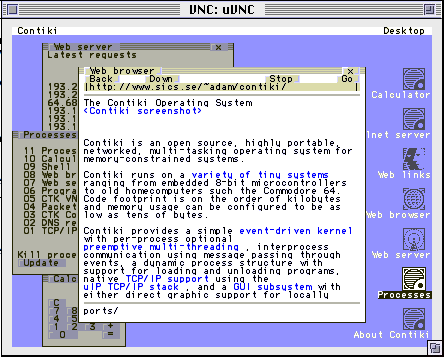
\includegraphics[width=9cm,keepaspectratio]{fig/contiki-vnc.png}
  \caption{Screenshot of running Contiki OS with CTK}
  \label{fig:contiki}
  \bigskip
\end{figure}


%=========================================================================
% (c) 2011, 2012 Josef Lusticky <xlusti00@stud.fit.vutbr.cz>

\section{Protothreads}\label{sec:contiki-protothreads}
Protothreads provide a way to run C functions quasi-paralelly, that is, a C functions work in a way similiar to thread.
In Contiki Protothreads allow process to wait for incoming events. While waiting for an event to occur another function
can be run. The core of this solution is C switch statement used in conjuction with variable (called local continuation)
containing the position where the function was interrupted. Next time function continues from this point.

The advantage of Protothreads over ordinary threads is that a Protothread does not require a separate stack.
In memory constrained systems, the overhead of allocating multiple stacks can consume large amounts of
the available memory. In contrast, each Protothread only requires few bytes for storing the state of execution.

A Protothread is driven by repeated calls to the function in which the Protothread is running.
Each time the
function is called, the Protothread will run until it blocks or exits.
Protothreads are implemented using local continuations. A local continuation represents the current state
of execution at a particular place in the program, but does not provide any call history or local variables.

The Protothreads API consists of four basic operations: initialization (PT\_INIT()), execution (PT\_BEGIN()),
conditional blocking (PT\_WAIT\_UNTIL()) and exit (PT\_END()). On top of these, two convenience functions
are built: reversed condition blocking (PT\_WAIT\_WHILE()) and Protothread blocking (PT\_WAIT\_THREAD())~\cite{paper-protothreads}.

To understand how are Protothreads implemented and how do the actually work please refer
to appendix~\ref{app:protothreads} in which an example of usage is shown.

Since Protothreads are implemented using standard C, library providing Protothreads can be used everywhere C toolchain is available.
But there are some cons to consider. Because protothreads are stackless, a Protothread can only run within a single C function.
There is also no way of storing automatic local variables. And since Protothreads are implemented using C {\it switch} statement, and these can
not be nested, the code that uses Protothreads cannot use {\it switch} statements itself.
Workaround for storing local variables is to prepend them with the {\it static} keyword, which make them being put into data segment
by compiler and thus remembering the value between the function calls.


%=========================================================================
% (c) 2011, 2012 Josef Lusticky

\section{uIP}\label{sec:contiki-uip}
The TCP/IP protocol suite is often used for communication over the Internet as well as local networks.
uIP (micro IP) is a complete TCP/IP communication stack developed by Adam Dunkels
for memory constrained systems such as embedded systems.

Before uIP, the TCP/IP architecture was considered to be heavyweight
due to its perceived need for processing power and memory.
The IP protocol was seen as too large to fit into the constrained environment -
existing implementations of the IP protocol family for general purpose computers would need hundreds
of kilobytes, whereas a typical constrained system has only a few tens of kilobytes of memory~\cite{interconnecting}.
For this reason, several non-IP stacks were developed.

In the early 2000's, however, this view was challenged by lightweight implementations of the IP
protocol family for smart objects such as the uIP stack~\cite{interconnecting}.
uIP showed that the IP architecture would fit nicely into the typical constrained systems,
without removing any of the essential mechanisms from IP.
Note that these resources, which are considered constrained today, are fairly close to the
resources of general purpose computers that were available when IP was designed~\cite{interconnecting}.
Since its initial release, the uIP stack has become widely used in networked
embedded systems~\cite{interconnecting, thesis-programming}.

uIP provides two different application programming interfaces to programmers:
a BSD sockets-like API called Protosockets and raw event-driven API.
Protosockets are based on Protothreads putting the same limitation on them - such as
no way of storing automatic local variables and an impossibility of using the C {\it switch} statement.
Protosockets only work with TCP connections~\cite{contiki-docs}.
Since NTP uses UDP, Protosockets will not be further
discussed in this thesis. For more information about Protosockets
please refer to the Contiki documentation~\cite{contiki-docs}.

uIP contains only the absolute minimum of required features to fulfill the protocol standard.
It can only handle a single network interface and contains the IP, ICMP, UDP and TCP protocols~\cite{contiki-docs}.
In order to reduce memory requirements and code size,
the uIP implementation uses an event-based API, which is fundamentally different
from the most common TCP/IP API, the BSD sockets API, present on Unix-like systems
and defined by the POSIX standard~\cite{thesis-programming,posix}.
An application is invoked in response to certain events and
it is up to the application that is receiving events from uIP to handle all
work with data to be transmitted. E.g. if the data is lost in the network,
the application will be invoked and then has to resend the data.
This approach is based on the fact that it should be simple for the application
to rebuild the same data.
This way, the uIP stack does not need to use explicit dynamic memory allocation.
Instead, it uses a single global buffer for holding packets and has a fixed
table for holding the connection state.
The global packet buffer is large enough to contain one packet of maximum size~\cite{contiki-docs}.

When a packet arrives from the network, the device driver places it in the
global buffer and calls the TCP/IP stack.
If the packet contains data, the TCP/IP stack will notify the corresponding application.
Because the data in the buffer will be overwritten by the next incoming packet,
the application will either have to act immediately on the data or copy the data into
its own buffer for later processing.
The packet buffer will not be overwritten by new packets before the application has processed the data~\cite{contiki-docs}.
Packets that arrive when the application is processing the data must be queued,
either by the network device or by the device driver.
That means uIP relies on the hardware when it comes to buffering.
Most single-chip Ethernet controllers have on-chip buffers
that are large enough to contain at least 4 maximum sized Ethernet frames~\cite{contiki-docs}.
This way, uIP does not have to have its own buffer structures and thus
only a minimal memory amount is required.
Possible packet loss is a trade-off for minimalism and ability to communicate using TCP/IP.
It is not such a big deal for communication using TCP on the transport layer
because of the acknowledgement scheme used in TCP to prevent data loss.
However data carried on UDP can be irrecoverably lost.

As was expected, measurements show that the uIP implementation provides very low
throughput, particularly when communicating with a PC host~\cite{thesis-towards}.
However, small systems that uIP is targeting, usually do not produce enough data
to make the performance degradation a serious problem~\cite{thesis-towards}.

Despite being so small, uIP is not only RFC compliant, but also IPv6 Ready Phase 1 certified.
uIP is written in the C programming language and it is fully integrated with the Contiki operating system.
In uIP, there are even some more tricks to shrink the stack
but complete uIP description is outside the scope of this thesis.
Please refer to the Contiki documentation for more details~\cite{contiki-docs}.


%=========================================================================
% (c) 2011, 2012 Josef Lusticky

\section{Kernel and processes}\label{sec:contiki-kernel}
The kernel in Contiki is event-driven providing cooperative multitasking
environment, but the system supports preemptive
multithreading that can be applied on a per-process basis~\cite{video}.
The preemption is not implemented in the kernel, but
preemptive multithreading is implemented as a library that is linked only with programs that
explicitly require multithreading~\cite{paper-contiki}.
The kernel itself contains no platform specific code, it implements only CPU multiplexing and
lets device drivers and applications communicate directly with hardware~\cite{video}.

From high level of abstraction,
applications in Contiki OS are implemented and run as processes.
Protothreads, the lightweight threads described in section~\ref{sec:contiki-protothreads},
are used in Contiki to implement processes.
Both the Contiki kernel and Contiki applications use
Protothreads extensively to achieve cooperative multitasking~\cite{contiki-wiki-faq}.
Every Contiki process consists of a process control block and a process thread~\cite{contiki-wiki-processes}.
The process control block contains run-time information about the process and
the process thread contains the code of the process.
Among other things, the process control block contains
textual name of the process, pointer to the process thread and state of the process.
The process thread is implemented as a single Protothread,
that is invoked from the process scheduler in the Contiki kernel~\cite{contiki-wiki-processes}.

From low level of abstraction,
every application is implemented as a simple C function
and the process control block remembers the actual state of execution of this function
in the same way as the local continuation works by Protothreads.
Processes are therefore running quasi-parallely in Contiki.

\bigskip
\begin{lstlisting}[caption=Process control block in Contiki OS]
struct process {
	struct process *next;
	const char *name;
	int (* thread)(struct pt *, process_event_t, process_data_t);
	struct pt pt;
	unsigned char state, needspoll;
	};
\end{lstlisting}

Process control block is not declared or defined directly,
but through the {\it{PROCESS()}} macro.
This macro takes two parameters: the variable name of the process control block
and a textual name of the process,
which is used in debugging and when printing out lists of active processes to users~\cite{contiki-wiki-processes}.

All code execution is initiated by the Contiki kernel
that acts like a simple dispatcher calling these functions~\cite{contiki-docs}.
Just like Protothreads, processes are also implemented using macros,
making them fully standard C compatible.

In Contiki, code run in either of two execution contexts:
cooperative, in which code never preempts other code, and preemptive,
which preempts the execution of cooperative code and returns control
when preemptive code is finished.
Processes always run in cooperative mode,
whereas interrupt service routines and real-time timers run in preemptive mode~\cite{contiki-wiki-processes}.
Code running in both execution contexts illustrates figure~\ref{fig:contiki-execution-context}.

\begin{figure}
  \centering
  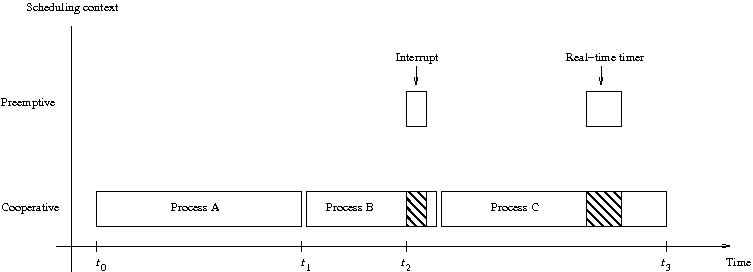
\includegraphics[width=13cm,keepaspectratio]{fig/Execution-contexts.png}
  \caption{Contiki execution contexts by A. Dunkels}
  \label{fig:contiki-execution-context}
\end{figure}

Interprocess communication is done by posting events in Contiki OS -
processes communicate with each other by posting events to each other~\cite{paper-contiki}.
There are two types of events: synchronous and asynchronous.
Synchronous events are directly delivered to the receiving process when posted and
can only be posted to a specific processes~\cite{contiki-wiki-processes}.
Because synchronous events are delivered immediately,
posting synchronous event is equivalent to a function call:
the process to which an event is delivered is directly invoked,
and the process that posted the event is blocked
until the receiving process has finished processing the event~\cite{contiki-wiki-processes}.

Asynchronous events are delivered to the receiving process
some time after they have been posted~\cite{contiki-wiki-processes}.
Before delivery, the asynchronous events are held on event queue inside Contiki kernel.
The kernel loops through this event queue and delivers
the event to the process by invoking the process. 
The receiver of an asynchronous event can be either a specific process
or all running processes~\cite{contiki-wiki-processes}.

%! paper-contiki - dunkels04contiki
%Being able to power down the device
%when the network is inactive is often required way to reduce energy consumption.
%Power conservation mechanisms
%depend on both the applications and the network protocols.
%The Contiki kernel contains no explicit power
%save abstractions, but lets the the application specific parts
%of the system implement such mechanisms.
%To help the application decide when to power down the system, the event
%scheduler exposes the size of the event queue.
%This information can be used to power down the processor when there
%are no events scheduled.
%! paper-contiki

%As stated before, Contiki is well documented and you can find out more about
%the kernel as well as the system in the documentation~\cite{contiki-docs}.


%=========================================================================
% (c) 2011, 2012 Josef Lusticky

\section{Timers}\label{sec:contiki-timers}
The Contiki kernel does not provide support for timed events,
instead an application that wants to use timers needs to explicitly use a timer library.
The timer library provides functions for setting, resetting and restarting timers,
and for checking if a timer has expired.
An application must manually check if its timers have expired - this is not done automatically~\cite{contiki-docs}.

Contiki has one clock library and a set of timer libraries: timer, stimer, ctimer, etimer, and rtimer~\cite{contiki-wiki-timers}.
The clock library provides functionality to handle the system time and to block the CPU for short time periods.
It is the interface between Contiki and the platform-specific hardware clock~\cite{contiki-docs}.
The timer libraries are implemented with the functionality of the clock library as a base~\cite{contiki-wiki-timers}.

The timer and stimer libraries provide the simplest form of timers and are used to check whether a time period has passed.
The difference between these two is the resolution of time -
timers use system clock ticks, whose value is incremented when an interrupt from the hardware clock occurs,
while stimers use seconds to offer much longer time periods~\cite{contiki-wiki-timers}.
The value representing seconds is also incremented in the interrupt service routine (ISR),
but only when enough clock ticks since last increment occurred.
The number of clock ticks within one second is represented by the
{\it{CLOCK\_SECOND}} macro provided by the clock library.
That means there are {\it{CLOCK\_SECOND}} interrupts from the hardware clock per second.
The usage of the timer library and {\it{CLOCK\_SECOND}} macro is shown in appendix~\ref{app:protothreads}.

The simplest timer and stimer libraries are not able to post an event when a timer expires.
Event timers should be used for this purpose.
Event timers (etimer library) provide a way to generate timed events.
An event timer will post an event to the process that set the timer when the
event timer expires~\cite{contiki-docs}.
The etimer library is implemented as a Contiki process and uses the timer library as a base.

Callback timers (ctimer library) provide a timer mechanism that calls a specified
C function when a ctimer expires~\cite{contiki-docs}.
Thus, they are especially useful in any code that does not have an
explicit Contiki process~\cite{contiki-wiki-timers}.

The Real-time timers (rtimer library) handle the scheduling and execution of
real-time tasks with predictable execution times~\cite{contiki-docs}.
The rtimer library provides real-time task support through callback functions -
the rtimer immediately preempts any running Contiki process in order to let the real-time tasks
execute at the scheduled time~\cite{contiki-wiki-timers}.
This behaviour is illustrated in figure~\ref{fig:contiki-execution-context}.
The rtimer library uses a separate hardware clock
to allow a higher clock resolution~\cite{contiki-wiki-timers}.
The small part of the rtimer library is architecture-agnostic,
but the particular implementation is platform-specific.



%=========================================================================
% (c) 2011, 2012 Josef Lusticky <xlusti00@stud.fit.vutbr.cz>

\chapter{Network Time Protocol}
Network Time Protocol provides mechanism for synchronising systems' clocks over the variable-latency data network.
% packet-oriented + citation
NTP was introduced and is still developed by David Mills at University of Delaware in Newark, United States.
NTP is argueably the longest running, continuously operating,
ubiquitously available protocol in the Internet~\cite{ntp-overview}.
Despite being one of the oldest surviving protocol on the Internet, it is not old-fashioned at all.
NTP version 4 described in RFC~5905~\cite{rfc5905} is an update to older NTPv3 to accomodate NTP to IPv6.
Version 4 also includes improvements in
the mitigation and discipline algorithms that extend
the potential accuracy to the tens of microseconds with modern
workstations and fast LANs~\cite{rfc5905}.
NTPv4 corrects some
errors in NTPv3 design and includes optional extension mechanism
that can be used for adding more capabilites to NTP, e.g. the
Autokey security protocol described in RFC~5906
for authenticating servers to clients.

Simple Network Time Protocol is simplified NTP implementation lacking complex
synchronisation algorithms used by NTP.
%citation  ?? ~\cite{rfc5905} ??
SNTP is also described in RFC 5905.
The packet of SNTP has the same structure and content as packet of NTP~\cite{rfc5905}.
From observing the network communication one can not tell whether the client
is full blown NTP implementation or just SNTP.
SNTP is a simplified sub-set of the algorithms used by the NTP protocol
making the client implementation not only easier, but also suitable for
resource constraint systems such as embedded systems.


%=========================================================================
% (c) 2011, 2012 Josef Lusticky

\section{Topology and hierarchy}\label{sec:ntp-topology}
NTP uses two different communication modes:
one to one, referred as unicast mode, and one to many, referred as broadcast mode~\cite{rfc5905}.
In unicast communication mode, NTP client sends request and NTP server sends response.
In broadcast communication mode, the client sends no request
and waits for a broadcast message from one or more servers~\cite{rfc5905}.

NTP servers are rated with stratum (plural form strata) number which represents their position
in an NTP hierarchy and their possible accuracy~\cite{rfc5905}.
Primary (stratum 1) servers synchronise to the reference clock directly traceable to UTC via
radio, satellite or modem.
The stratum 2 servers synchronise to stratum 1
servers via hierarchical subnet.
The stratum 3 servers synchronise to stratum 2 servers, and so on.
The maximum stratum is 15, number 16 means unsynchronised server
and higher numbers (up to 255) are reserved~\cite{rfc5905}.
Synchronisation between servers in the same stratum level is also possible.
Figure~\ref{fig:ntp-hierarchy} shows a brief hierarchy of NTP.
\begin{figure}
  \centering
  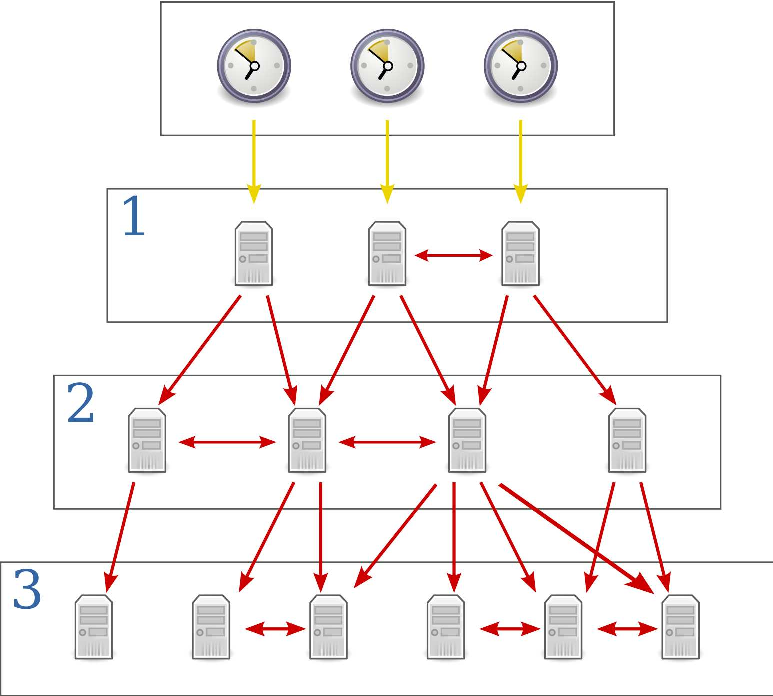
\includegraphics[width=9cm,keepaspectratio]{fig/Network_Time_Protocol_servers_and_clients.pdf}
  \caption{Topology and hierarchy of NTP by B. Esham}
  \label{fig:ntp-hierarchy}
  \bigskip
\end{figure}


%=========================================================================
% (c) 2011, 2012 Josef Lusticky <xlusti00@stud.fit.vutbr.cz>

\section{Time and timescales}\label{sec:ntp-time}
For expressing the time NTP always uses the Coordinated Universal Time (UTC)~\cite{rfc5905}.
UTC is maintained by the International Bureau of Weights and Measures in Paris, France.
It is the time scale that forms the basis for coordinated dissemination
of standard frequencies and time signals~\cite{bipm-utc}.
The time specified by UTC is the same for all timezones.
Its calculation is the same as with Greenwich Mean Time (GMT),
however the daylight savings are not accounted.

The UTC scale is adjusted by the insertion of leap seconds to ensure approximate
agreement with the time derived from the rotation of the Earth~\cite{bipm-utc}.
The atomic clocks, on which UTC is based, are so precise that
they do not match the rotation of the Earth,
which periodically speeds up and slows down due to the action
of tides and changes within the Earth's core~\cite{cnn-earth}.
The goal of a leap second is to catch up UTC with these changes.
The leap second is inserted or deleted on the advice of
International Earth Rotation and Reference Systems Service~\cite{bipm-utc}.
NTP is well designed for leap second occurrence -
there is Leap Indicator field
in the structure of NTP packet and there are also fields intended for
information about leap second in structures that NTP algorithm uses~\cite{rfc5905}.
The formal definition of UTC does not permit double leap seconds~\cite{posix}.

In computer the system time is represented by system clock maintained by
hardware and operating system.
The goal of the NTP algorithms is to minimize
both the time difference and frequency difference between UTC and the system clock.
When these differences have been reduced below nominal
tolerances, the system clock is said to be synchronised to UTC~\cite{rfc5905}.
It has never been a goal of NTP to take care of local time,
it is up to operating system to provide user the correct local time~\cite{ntp-overview}.

The NTP and POSIX timescales are based on the UTC timescale,
but not always coincident with it~\cite{ntp-leap}.
Both timescales reckon in seconds since the prime epoch,
but the origin of the NTP timescale, the NTP prime epoch, is 00:00:00 UTC on 1 January 1900,
while the prime epoch of the POSIX timescale is 00:00:00 UTC on 1st January 1970~\cite{ntp-leap}.
%! VYHODIT?
So upon the first tick of POSIX clock on 1st January 1970 the NTP clock read 2~208~988~800,
representing the number of seconds since the NTP prime epoch.
Some of interesting dates with their respective NTP time values
can be found in appendix~\ref{app:dates}.


%=========================================================================
% (c) 2011, 2012 Josef Lusticky <xlusti00@stud.fit.vutbr.cz>

\section{Network and timestamps}\label{sec:ntp-network}
Network specification of NTP defines that
the protocol uses the User Datagram Protocol (UDP) on port number 123~\cite{ianna-ports,rfc5905}.
Reliable message delivery such as TCP can actually make the delivered NTP packet less reliable since retries
would increase the delay value and other errors~\cite{rfc5905}.
This is mostly due to overhead of communication with TCP on transport layer.

NTP manipulates with the time through timestamps - a record of time.
NTP timestamp has two fields. The seconds field expressing the number of seconds
and the fraction field expressing fraction of a second~\cite{rfc5905}.
All NTP time values are represented in twos-complement format, with
bits numbered in big-endian fashion from zero starting at the left, or high-order, position~\cite{rfc5905}. 
There are two formats of timestamp in NTP packet structure:
long 64-bit and short 32-bit as shown on figure~\ref{fig:ntp-timestamps}.
The 64-bit long timestamp used by NTP consists of a 32-bit unsigned seconds
field spanning $2^{32}$ seconds (aprox. 136 years from 1900 to 2036) and a 32-bit fraction field resolving
$2^{-32}$ seconds (aprox. 232 picoseconds)~\cite{rfc5905}.
The short 32-bit timestamp includes a 16-bit unsigned seconds field
and 16-bit fraction field.

There is one more NTP time format - 128-bit date format.
This format is however not transmitted over the network
and since this 128-bit date format is used where sufficient storage and word
size are available~\cite{rfc5905},
there is practically no need of knowing about this format for embedded systems.
But strictly speaking an NTP timestamp is a truncated NTP date format~\cite{rfc5905}.

\begin{figure}
	\centering
	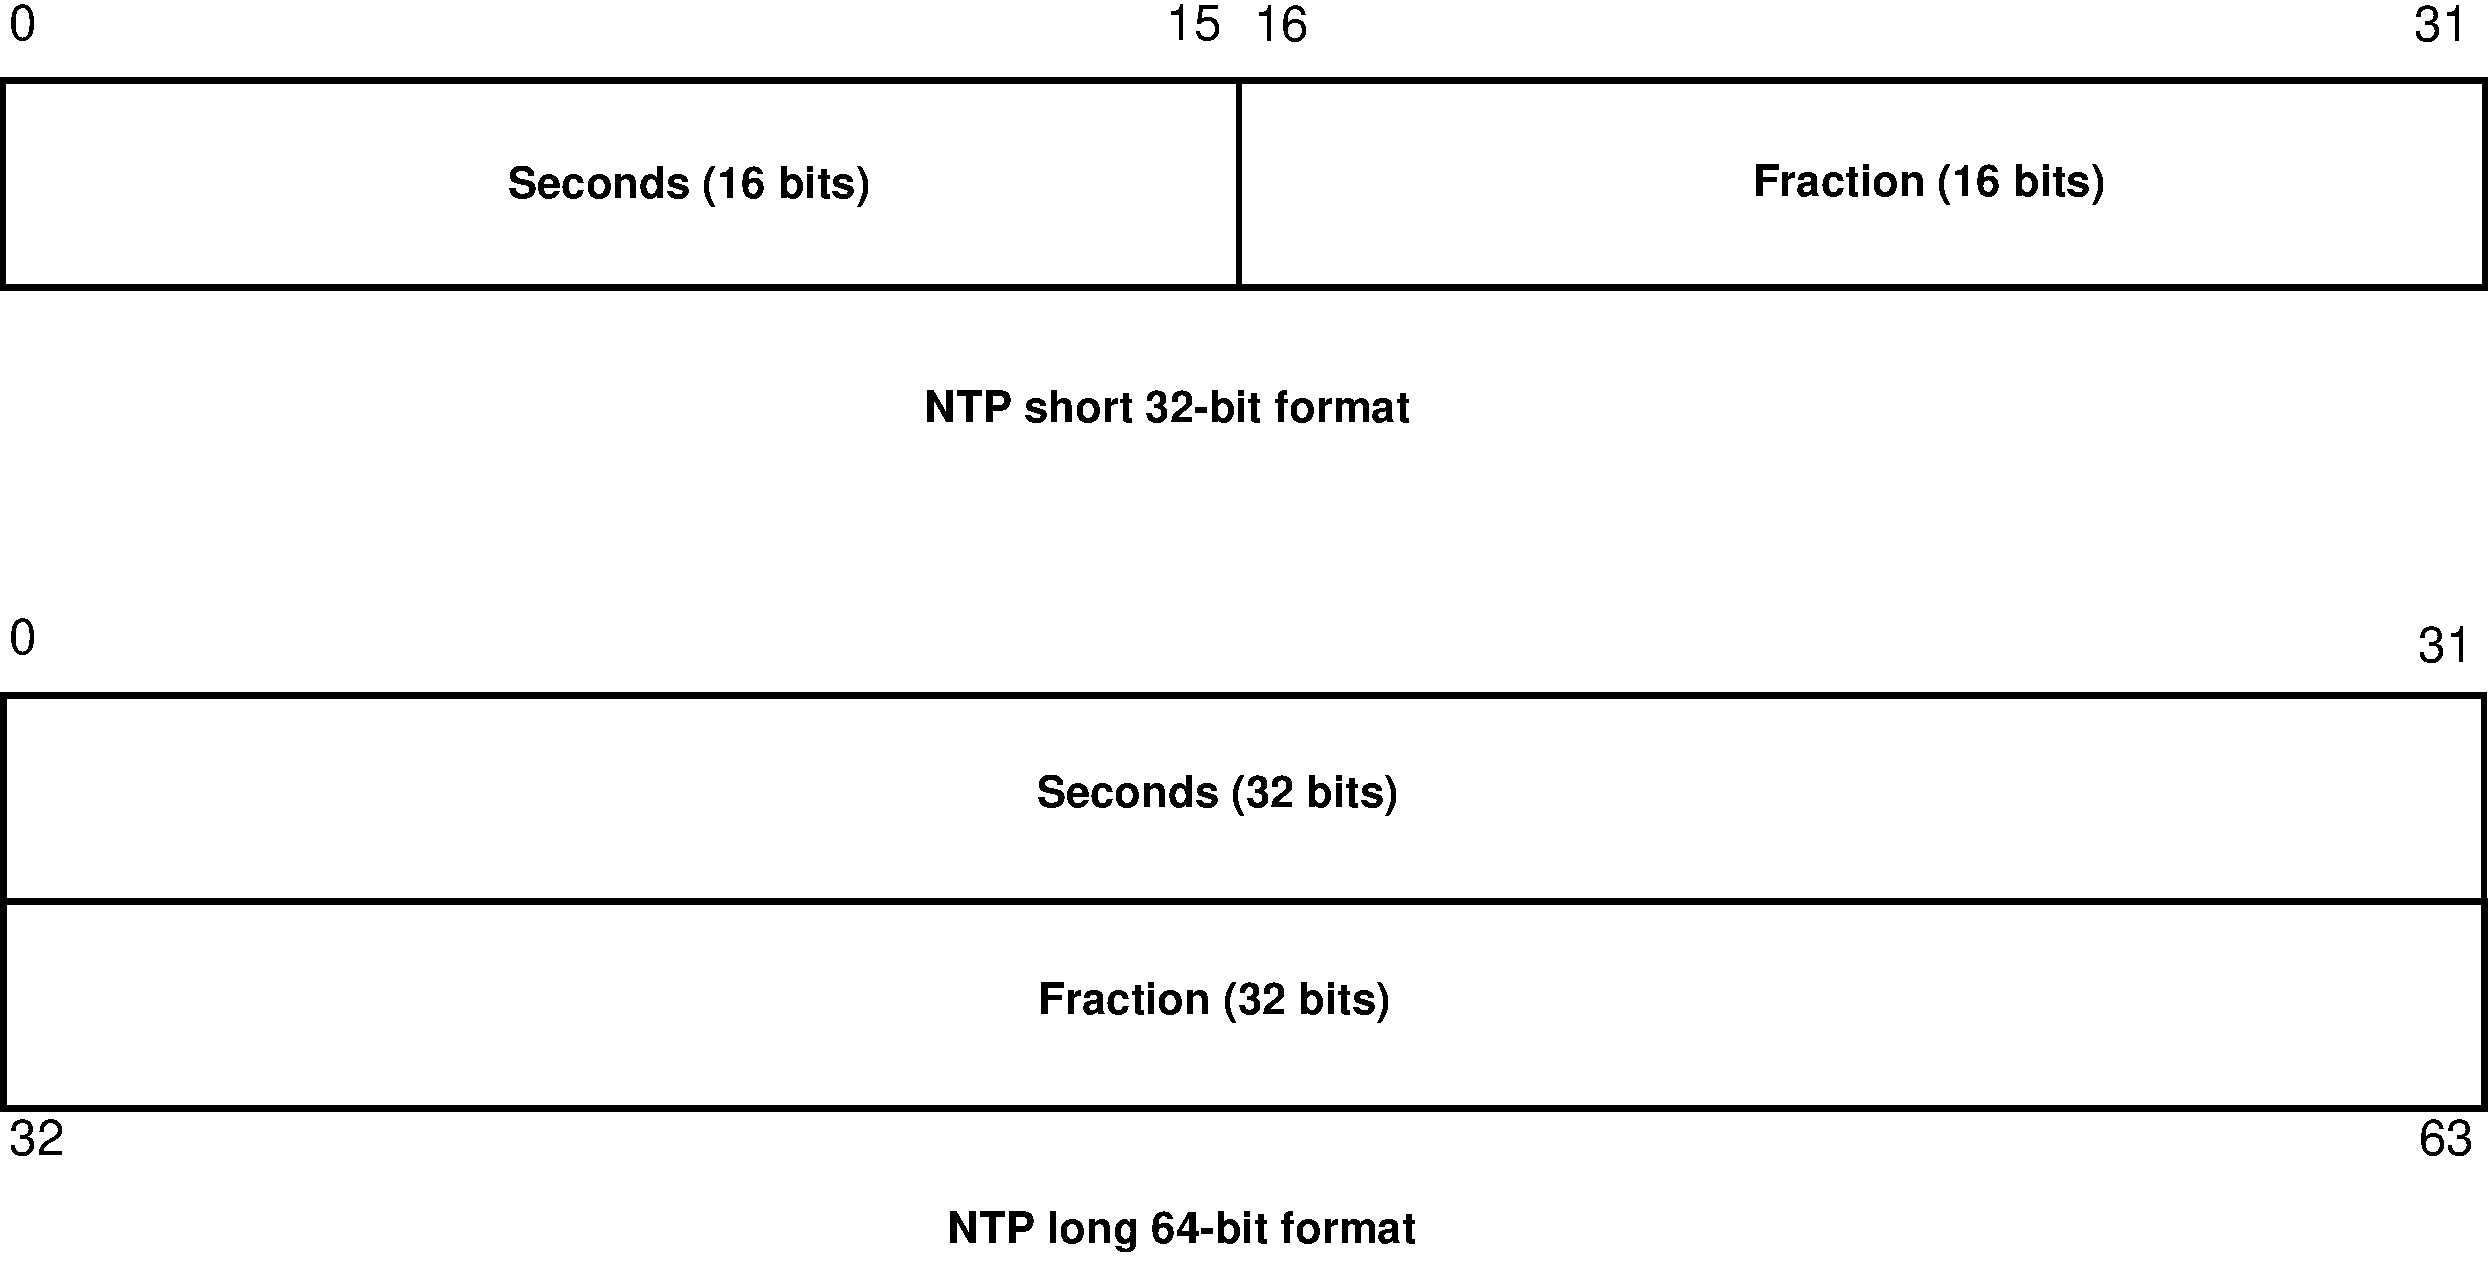
\includegraphics[width=13cm,keepaspectratio]{fig/ntp-timestamps.pdf}
	\caption{Time formats used in NTP packet}
	\label{fig:ntp-timestamps}
	\bigskip
\end{figure}

% TODO - packet

\begin{figure}
	\centering
	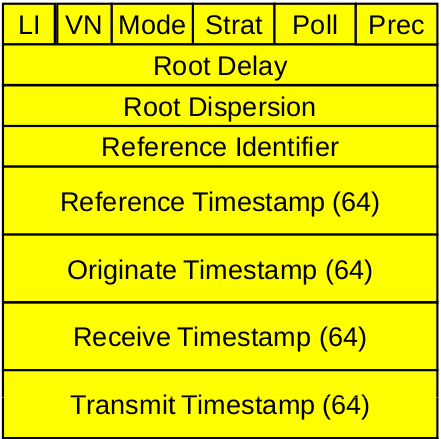
\includegraphics[width=6cm,keepaspectratio]{fig/ntp-packet.png}
	\caption{Basic NTP packet structure}
	\label{fig:ntp-packet}
	\bigskip
\end{figure}


Because the short 32-bit format is used for Root dispersion and Root Delay fields,
they do not need so big scope and precision.
Root dispersion express accumulated total dispersion from primary server
and Root Delay express accumulated roundtrip delay via primary server~\cite{ntp-arch}.

%TODO

Because of network latency the timestamp recieved will never be exactly corresponding to
the current time.
One of the main goals of NTP is to deal with the network latency~\cite{ntp-overview}.



%=========================================================================
% (c) 2011, 2012 Josef Lusticky

\section{Algorithms}\label{sec:ntp-algorithms}
Because of network latency the received Transmit Timestamp will never be exactly
corresponding to the current time.
One of the main goals of NTP is to deal with the network latency~\cite{ntp-overview}.

As described in section~\ref{sec:ntp-network},
there are the following 64-bit long timestamps in NTP packet: Origin, Receive and Transmit Timestamp.
Upon NTP packet arrival, the client determines another timestamp called
Destination Timestamp~\cite{rfc5905}.
This timestamp is represented as T4 on figure~\ref{fig:ntp-client-server}
and is not part of NTP packet structure.

Using these four timestamps, NTP client using unicast communication mode can compute
the local clock offset which is given by $\theta = \frac{1}{2}[(t_2 - t_1) + (t_3 - t_4)]$,
where $t_1$ is the time of the request packet transmission (Origin Timestamp),
$t_2$ is the time of the request packet reception (Receive Timestamp),
$t_3$ is the time of the response packet transmission (Transmit Timestamp) and
$t_4$ is the time of the response packet reception (Destination Timestamp)~\cite{ntp-algor,rfc5905}.
The implicit assumption in the above is that one-way delay is
statistically half of round-trip delay~\cite{rfc5905},
which is given by $\delta = (t_4 - t_1) - (t_3 - t_2)$.

In broadcast communication mode, Origin and Receive Timestamps are not accounted.
The client computes its local clock offset which is given by $\theta = t_3 - t_4$.
The implicit assumption in the above is that one-way delay from server to client is zero.
Since this is never the case, it is useful to provide an
initial volley where the client exchanges several packets with the server in
order to calibrate the propagation delay~\cite{rfc5905}.

When computing the result from more servers, the intersection algorithm is used
for selecting the possible most exact timestamp received from various servers~\cite{ntp-improved-algor,rfc5905}.
Intersection algorithm is derived from Murzollo algorithm but the basic
computation remains the same~\cite{ntp-history}.
First of all a selection of bad and good servers must be made.
Bad servers are called Falsetickers and good are called Truechimers~\cite{rfc5905}.
The division to these sets is based on their response.
As one can assume for a sensible result there must be more Truechimers than Falsetickers~\cite{rfc5905}.

After selecting a set of reliable servers, NTP clock algorithms compute resulting exact timestamp.
The resulting exact timestamp does not have to be the same
as one of those provided by the servers.
NTP clock algorithms calculate using clock accuracy estimates
determined from Root Dispersion, Root Delay and Precision fields of server's response.
These estimates are converted to intervals.
Figure~\ref{fig:ntp-intersection} shows the computation for the following example:
If we have the estimates $10 \pm 2$, $12 \pm 1$ and $11 \pm 1$
then these intervals are $<8; 12>$, $<11; 13>$ and $<10; 12>$ which
intersect to form $<11; 12>$ or $11.5 \pm 0.5$ as consistent with all three values.
The arithmetic mean is used as the result value.
When querying servers again, the algorithm repeats but the new result computation
also depends on the previous result~\cite{rfc5905,ntp-history}.
This eliminates possible jitter which can be caused by repeatedly querying the servers
and getting slightly different answers from them.

\begin{figure}
	\centering
	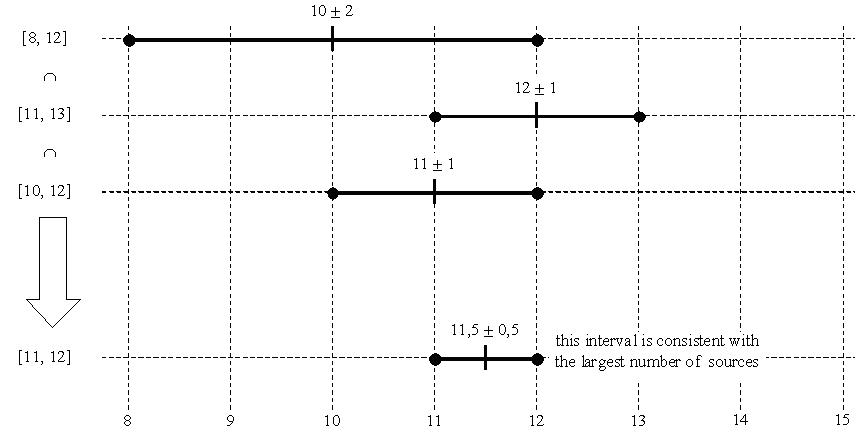
\includegraphics[width=13cm,keepaspectratio]{fig/Marzullo_example-1.jpg}
	\caption{Intersection algorithm by D. Exb}
	\label{fig:ntp-intersection}
	\bigskip
\end{figure}

%Since the clients complying with a subset of NTP, called
%the Simple Network Time Protocol (SNTPv4) [RFC4330], do not need to
%implement the mitigation algorithms ... ~\cite{rfc5905}.



\section{Hardware concerns for implementing real-time support}
A typical desktop computer today includes CPU based on Intel x86 architecture.
Real-Time Clock (RTC) in CMOS memory that is battery powered

Unfortunately Intel x86 architecture is heavily influenced by backwards compatibility,
e.g. the time value can also be stored in Binary Code Digit (BCD) encoding in RTC.

In year 19xx / Starting with Intel 386
Intel introduced
PIT Intel 8253 and 8254 - 3 counters (counter 0 interrupt to OS)


Used by historic versions of Linux
=> read initial time from RTC, setup PIT and interrupts (IRQ 0, INT 8), increment jiffies on every interrupt, provide app resolution of jiffies

init/main.c - time\_init() - read from RTC and save to startup\_time
kernel/sched.c - sched\_init() = PTI setup for interrupts - LATCH (1193180/HZ)
kernel/system\_call.s - timer\_interrupt() in assembly - increments jiffies

The current real time is provided by CURRENT\_TIME (startup\_time+jiffies/HZ) => since jiffies is integer and HZ is 100 => resolution of 10ms.
kernel/sys.c - sys\_time() - CURRENT\_TIME returned


\section{NTP on POSIX-compliant systems}
Operating systems
Linux
OpenBSD
DragonflyBSD

NTP implementations
NTP from ntp.org project - reference implementation
Chrony
OpenNTPD - OpenBSD
dntpd - DragonflyBSD



%=========================================================================
% (c) 2011, 2012 Josef Lusticky

\chapter{Analysis}
For implementation of a reasonably useful NTP client,
an operating system must be able to set, get and eventually adjust the system time.
Though not mandatory, adjusting the time is an important function,
if the time shall be always a monotonically increasing function.
Apart from that, ability to communicate over UDP is also required.

For developing and testing Contiki NTP Client,
the AVR Raven platform with 8-bit ATmega1284P CPU~\cite{avr-datasheet} will be used.
This platform features IEEE~802.15.4 (Low-Rate Wireless Personal Area Networks) link layer support.
Together with an adaptation layer called 6LoWPAN (IPv6 over Low power Wireless Personal Area Networks),
AVR Raven is able to communicate over IPv6.

%=========================================================================
% (c) 2011, 2012 Josef Lusticky

\section{Time interface}\label{sec:analysis-time}
For keeping, measuring and resolving the time computer needs a clock.
A computer clock is an electronic device with a counter register counting oscillations in a
quartz crystal oscillator with a particular frequency~\cite{thesis-sync}.
The structure of the clock hardware is shown in figure~\ref{fig:system-hardware-clock}.
\begin{figure}
  \centering
  
\includegraphics[width=9cm,keepaspectratio]{fig/pc-clock.png}
  \caption{A typical hardware clock (source:~\cite{thesis-beat})}
  \label{fig:system-hardware-clock}
\end{figure}
When the counter reaches a specific value, an interrupt is generated and the counter register is reset.
Such interrupt is called {\it{clock tick}}, or {\it{timer tick}}, and at each clock tick,
interrupt service routine increments a system clock value stored in the memory~\cite{thesis-sync}.
In a typical computer clock design, interrupts are produced at
fixed tick intervals in the range 1-20~ms~\cite{nanokernel}.

In Contiki, such a design is used by the clock library, described in section~\ref{sec:contiki-timers}.
There is a variable counting clock ticks, called {\it{scount}},
and a variable counting seconds, called {\it{seconds}}.
As described in section~\ref{sec:contiki-timers}, there are
exactly {\it{CLOCK\_SECOND}} ticks in one second.
When the {\it{scount}} variable reaches this value,
the {\it{seconds}} variable is incremented and the {\it{scount}} variable is reset.
Both variables are used by the Contiki timers discussed in section~\ref{sec:contiki-timers}.

Since the value of the {\it{seconds}} variable is zero after the system booted,
it actually expresses the system uptime.
The {\it{seconds}} variable can be read by the application using the {\it{clock\_seconds}} call.
However, in Contiki 2.5 there is no call for setting this variable.
In the current Git version at the time of writing, a new call {\it{clock\_set\_seconds}}
can be used for this purpose.
Because this call simply rewrites the {\it{seconds}} variable, it breaks the stimer library,
and should by avoided by the NTP client.
%The {\it{clock_set_seconds}} call is implemented only for three CPU architectures at the time of writing.

The precision of one second is also not adequate for the NTP client.
Further precision can be acquired by reading the {\it{scount}} variable,
as it provides resolution of $\frac{1}{CLOCK\_SECOND}$.
Moreover, the hardware counter can be also queried, as it includes the time passed since
the last update of the {\it{scount}} variable.
If stimers should not be broken by setting the {\it{seconds}} variable,
and Contiki should be able to set and provide the current time in a higher precision,
a new call interface must be developed.

Similarly, there is no call for adjusting the time in Contiki.
Due to memory constraints, software structures controlling the time adjustments are too heavyweight
for a usage in an embedded operating system.
Due to lower CPU frequencies, the code of an interrupt service routine can not be complex
and sophisticated clock discipline algorithms should be avoided.
Because of this, a call for adjusting the time should use abilities
provided by the hardware clock as much as possible.


%=========================================================================
% (c) 2011, 2012 Josef Lusticky

\section{Clock subsystem}\label{sec:analysis-clock}
Contiki provides a basic clock interface particularly for use of timers
with a simple goal - measuring time.
This interface is common for all supported platforms,
but the particular implementation is platform specific.
The definition of the common interface is located in the {\it{core/sys/clock.h}} file
and the specific implementations can be found in the {\it{clock.c}} file
in {\it{cpu/}} directory of the Contiki source code.

The clock interface provides the {\it{clock\_init}} call for initialising the hardware clock,
that is automatically called during the boot sequence of Contiki.
The {\it{clock\_init}} call sets up
appropriate registers and the interrupt service routine as described in section~\ref{sec:analysis-clock}.
This call is implemented as the C macro for AVR CPUs, that evaluates to a specific setup code for each
different AVR CPU during the compilation, and is defined in the {\it{cpu/avr/dev/clock-avr.h}} file.
The setup code is not common to all AVR CPUs because of differences among them - e.g. there are usually
only three Timer/Counter modules, but AVR ATmega1284P has four Timer/Counter modules~\cite{avr-datasheet}.

On AVR Raven, 8 bit Timer/Counter~2 clocked from asynchronous 32~768~Hz crystal oscillator
is used by default by Contiki clock interface.
This oscillator is independent of any other clock,
can be only used with Timer/Counter~2 and it
enables use of Timer/Counter~2 as a Real Time Counter~\cite{avr-datasheet}.
The Timer/Counter~2 prescale value 8 is used in Contiki on AVR Raven platform -
the oscillator frequency of 32~768~Hz is effectively divided by 8.
The counter register is hence incremented with the frequency of
$f_{T2} = {\frac{f_{asy}}{prescaler}} = {\frac{32768}{8}} = 4096$~Hz.
Figure~\ref{fig:avr-clock} shows the Timer/Counter~2 clock module.
\begin{figure}
  \centering
  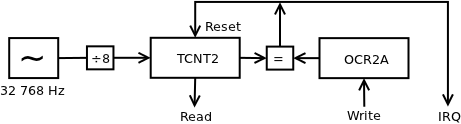
\includegraphics[width=9cm,keepaspectratio]{fig/avr-clock.png}
  \caption{Timer/Counter 2 hardware clock module on AVR Raven}
  \label{fig:avr-clock}
\end{figure}

%%Unlike I/O clock used for clocking other Timers/Counters,
%%this asynchronous crystal is also active in power-save mode~\ref{avr-datasheet}.
%CITATION: If Timer/Counter2 is enabled, it will keep running during sleep. The device can wake up from
%either Timer Overflow or Output Compare event from Timer/Counter2.
%If Timer/Counter2 is not running, Power-down mode is recommended instead of Power-save
%mode.
%The Timer/Counter2 can be clocked both synchronously and asynchronously in Power-save
%mode. If the Timer/Counter2 is not using the asynchronous clock, the Timer/Counter Oscillator is
%stopped during sleep. If the Timer/Counter2 is not using the synchronous clock, the clock source
%is stopped during sleep. Note that even if the synchronous clock is running in Power-save, this
%clock is only available for the Timer/Counter2.

The Timer/Counter~2 module is used in the Clear Timer on Compare Match (CTC) mode by Contiki.
In this mode, the counter register {\it{TCNT2}} is incrementing
and the compare register {\it{OCR2A}} defines the maximum value of the counter register.
Compare match between the counter register and the compare register
sets the Output Compare Flag {\it{OCF2A}} and resets the counter register to zero~\cite{avr-datasheet}.
This behaviour is illustrated in figure~\ref{fig:design-timing-diagram}
- the {\it{TOP}} value is equal to the value in the compare register and the {\it{BOTTOM}} value is equal to zero.

\begin{figure}
  \centering
  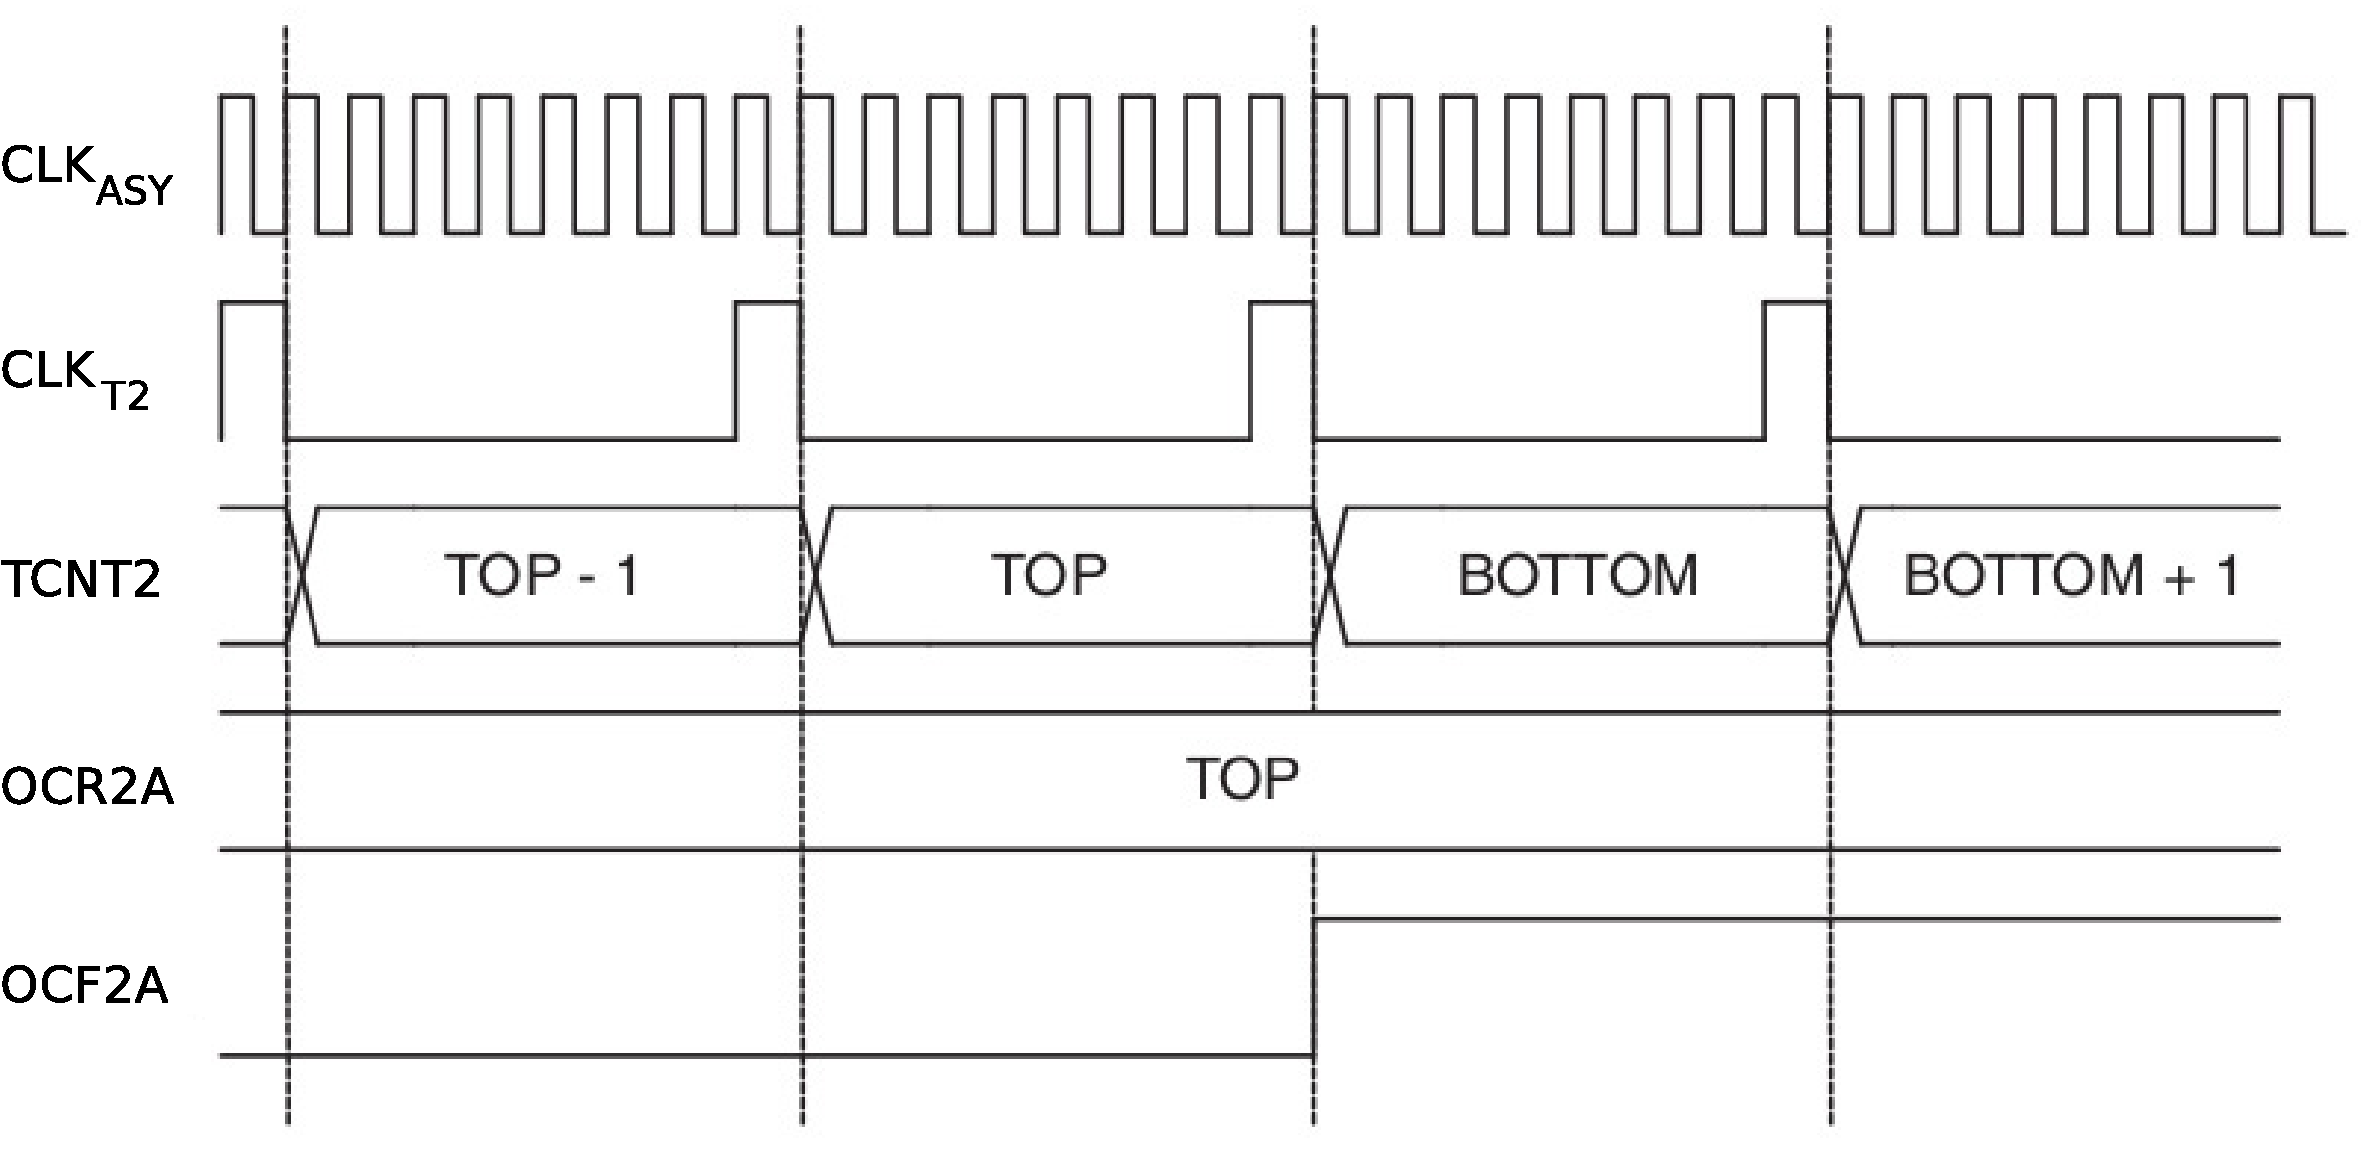
\includegraphics[width=12cm,keepaspectratio]{fig/timing-diagram.pdf}
  \caption{Timing diagram in CTC mode with prescaler 8 (source:~\cite{avr-datasheet})}
  \label{fig:design-timing-diagram}
\end{figure}

Additionally, when compare match occurs,
an interrupt is raised and the interrupt service routine {\it{AVR\_OUTPUT\_COMPARE\_INT}},
defined in {\it{cpu/avr/dev/clock.c}} file, is executed.
The flag indicating occurred match {\it{OCF2A}} is
cleared automatically by hardware when executing
the interrupt service routine in this case~\cite{avr-datasheet}.

To obtain {\it{CLOCK\_SECOND}} interrupts per second, there must be
${\frac{f_{T2}}{CLOCK\_SECOND}}$ hardware clock ticks between two successive interrupts.
On compare match in CTC mode, the timer is reset to zero as
shown in figure~\ref{fig:design-timing-diagram}.
The value zero is also included in the counting - the 0th count of the timer also takes one tick.
Therefore the value of compare register {\it{OCR2A}} must be ${\frac{f_{T2}}{CLOCK\_SECOND}} - 1$
when using Timer/Counter~2 in CTC mode.
The default value of {\it{CLOCK\_SECOND}} for AVR Raven in Contiki is 128,
which implies the default value of the compare register ${\frac{4096}{128}} - 1 = 31$.
The {\it{CLOCK\_SECOND}} value is defined in {\it{platform/avr-raven/contiki-conf.h}} file
and the default value of the compare register is computed during the compilation.

The interrupt service routine can be further used for updating the value in {\it{OCR2A}} compare register.
This can be used for adjusting the time, because decrementing the compare register
value causes a faster increment of the {\it{scount}} variable, which in turn causes
a faster increment of the {\it{seconds}} variable and vice versa.
However, changing {\it{OCR2A}} to a value closer to zero when the counter is running
must be done with care since the CTC mode does not have a double buffering feature.
If the new value written to {\it{OCR2A}} is lower than the current
value of {\it{TCNT2}}, the counter will miss the compare match~\cite{avr-datasheet}.



\section{Communication}
Without any NTP server is an NTP client useless. % There are clients, servers...
However, too many server associations complicate the client design.
In fact, in the most common scenario, there can be only a single NTP master server
for the whole network.
A single server association requires just a simple calculation of the local clock offset
$\theta$, whereas more server associations require the intersection algorithm,
described in section~\ref{sec:ntp-algorithms}.
Implementation of such an algorithm, requiring advanced data structures, should be avoided
in a memory constrained system.

The NTP broadcast communication mode, on the other hand,
requires no associations and no packet filling process on the client side.
Moreover, because the client does not have to actively send any NTP packets,
an energy consumption of the client is reduced.

% 1 - see design
A problem might be a possible packet loss when communication uses UDP on transport layer.
The reason why this can happen often in Contiki, is explained in section~\ref{sec:contiki-uip}.
% 2
In NTP unicast mode, the packet loss might occur either for a client's query to the server
or for a server's response to the client.
If the client's query loss occurs, no server response will be sent.
Similarly, if the server's response loss occurs, no message will be received by the client.
Not to block a whole system till the response arrives
is therefore a desired behaviour of the client.

The NTP client should be able to communicate over both IPv4 and IPv6.
Thanks to the uIP stack, this is no a matter for Contiki.
The only constraint is that both IP versions can not be used simultaneously
and the decision must be made during the compilation~\cite{contiki-docs}.
Although the {\it{UIP\_CONF\_IPV6}} macro can be used to determine which IP version
support is being compiled, the NTP client application can be written IP-version agnostic.


\section{Timestamp conversions}%CLIENT CODE
As mentioned in section~\ref{sec:ntp-time}, the NTP timescale is not
coincident with the POSIX timescale.
If the new call interface should use the standard POSIX timescale,
conversion between NTP and POSIX timestamps must be calculated.
The conversion from the POSIX timestamp to the 64-bit long NTP timestamp
is needed when the client sends the request
and the conversion vice versa is needed when the client calculates
the local clock offset from the received timestamps.

Since both timescales reckon in seconds, the conversion between
the NTP timestamp seconds field value and the POSIX timestamp seconds field value is simple.
However, the conversion between the NTP fraction field value ($2^{-32}$)
and the POSIX fraction field value (nanoseconds or microseconds) is problematic.
The relation between the POSIX fraction field and the NTP fraction field
is given by $POSIX.frac = NTP.frac \times POSIX.res \div 2^{32}$,
where $POSIX.frac$ is the POSIX fraction field value,
$NTP.frac$ is the NTP fraction field value and
$POSIX.res$ is the POSIX timestamp resolution (microseconds or nanoseconds).
The accurate conversion requires either floating point operations or operations with 64 bit numbers.
These operations can be memory expensive, especially on 8-bit microcontrollers,
and their usage must be considered carefully or another suitable solution must be found.


%Operating system maintains the current time and advances it at every interrupt.



%Such a design is also used by the timer library in Contiki~\cite{contiki-docs}.

%Because of the speed requirement,
%the system time uses a linear time scale like seconds
%(instead of dealing with seconds, minutes, hours, days, etc.)
%and only if a human is in need of the current time,
%the system time is converted~\cite{ntp-faq}.




%\section{Clock quality factors}
%Unfortunately all the common clock hardware is not very accurate~\cite{ntp-faq}.
%This is simply because the frequency that makes time increase is never exactly right.
%Even an error of only 0.001\% would make a clock be off by almost one second per day.
%Almost every clock can have unique behaviour depending on many conditions~\cite{ntp-faq}.
%The following factors are therefore used for expressing clock quality and behaviour:
%\begin{itemize}
%\item
%Frequency is the rate at which a clock progresses~\cite{thesis-sync}.
%\item
%It is sometimes convenient
%to express frequency offsets in parts-per-million~(PPM), where~1~PPM
%is equal to $10^{-6}$ $\frac{s}{s}$ (0.0001\%)~\cite{rfc5905}.
%\item
%From long-term observation one may also notice variations in the clock frequency.
%The difference of the frequency is called wander~\cite{ntp-faq}.
%There can be clocks with poor short-term stability, but with good long-term stability, and vice versa.
%\item
%Resolution is the smallest possible increase of time the clock model allows.
%If a clock increments its value only once per second, its resolution is also one second~\cite{ntp-faq}.
%\item
%Precision is the smallest possible increase of time that can be experienced
%by a program~\cite{ntp-faq}.
%\item
%When repeatedly reading the time, the difference may vary almost randomly.
%The difference of these differences (second derivation) is called jitter~\cite{ntp-faq}.
%\item
%Accuracy determines how close the clock is to an official time reference~\cite{ntp-faq}.
%\item
%Offset is the difference between the time read by the clock and the reference time~\cite{thesis-sync}.
%\item
%Reliability determines the time a clock can keep within a specified accuracy~\cite{ntp-faq}.
%\end{itemize}

%As mentioned before, all of the common hardware clocks are not very accurate.
%Real clocks have a frequency error of several PPM quite frequently
%and some of the best clocks available still have errors of about $1^{-8}$PPM~\cite{ntp-faq}.
%Even if the systematic error of some clock model is known, the clock will never be perfect.
%This is because the frequency varies over time, mostly influenced by temperature,
%but it could also be air pressure or magnetic fields~\cite{ntp-faq}.

%\section{Clock discipline}\label{sec:system-discipline}
%For keeping an accurate time a clock not only needs to be read, it must be also set.
%However, simply setting the clock to remove the offset would cause unpredictable time steps~\cite{ntp-faq}.
%Since real time is an always monotonically increasing function, this is not a desired behaviour~\cite{ntp-faq}.
%For minimising the time offset and frequency difference between
%the reference clock and the local clock without any time step, an NTP client can be used.

%With the current system time knowledge and the local clock offset knowledge,
%an NTP client can compute an amount of adjustments needed to synchronise the local clock.
%To apply these adjustments, operating system must also provide a call
%for adjusting the time (usually called {\it{adjtime}})~\cite{nanokernel}.
%This call speeds up or slows down the system time in order to synchronise the local clock.
%Periodical application of such corrections {\it{disciplines}} the local clock~\cite{ntp-faq}.

%However, some clock implementations do not allow small corrections to be applied
%to the system clock, and there is also no standard interface to monitor the system clock's quality~\cite{ntp-faq}.
%This was the main reason for developing a new kernel clock model called {\it{Kernel discipline}}~\cite{nanokernel}.
%The new kernel clock model provides improved time and frequency
%resolution, together with a more agile and precise clock discipline mechanism~\cite{nanokernel}.
%This model is described in RFC~1589~\cite{rfc1589} and it adds new calls to the existing kernel interface
%{\it{ntp\_gettime}}, {\it{ntp\_settime}} and {\it{ntp\_adjtime}}.
%Apart from the system time, these calls also provide maximum error (synchronisation distance)
%and estimated error (dispersion) to client user application programs, such as NTP client~\cite{rfc1589}.
%The programming interface also includes the new
%system call {\it{ntp\_adjtime}} mentioned previously, which can be used
%to read and write kernel variables for time and frequency
%adjustment, leap-second warning and related data~\cite{rfc1589}.
%The clock corrections are calculated and applied inside the kernel~\cite{ntp-faq}.

%%!TODO
%Both of the models have benefits and drawbacks,
%but further description of them is outside the scope of this thesis.
%These are further discussed, particularly in relation to Contiki~OS, in %chapter~\ref{}.


%=========================================================================
% (c) 2011, 2012 Josef Lusticky

\chapter{Design and analysis}
For implementation of reasonably useful NTP client,
operating system must be able to set, get
and eventually adjust the system time in a similar fashion as
described in section~\ref{sec:system-keeping-and-providing} and~\ref{sec:system-discipline}.
Though not mandatory, adjusting time is important function,
if the time shall be always a monotonically increasing function.
Apart from that, communicating abilities over UDP are also required.

For developing and testing Contiki NTP client,
the AVR Raven platform with 8-bit ATmega1284P CPU~\cite{avr-datasheet} will be used.
This platform features IEEE~802.15.4 (Low-Rate Wireless Personal Area Networks) link layer support.
Together with an adaptation layer called 6LoWPAN (IPv6 over Low power Wireless Personal Area Networks)
AVR Raven is able to communicate over IPv6.

How to get a working setup with Contiki on this platform is described in
the document files on the CD enclosed to this thesis.
The CD content hierarchy is listed in appendix~\ref{app:cd-content}.

%... This is not in Contiki, as operating systems targeted at embbeded systems produce only 1 binary file. CITATION

%=========================================================================
% (c) 2011, 2012 Josef Lusticky

\section{Network communication}
Thanks to uIP, described in section~\ref{sec:contiki-uip},
the network communication is not a matter for Contiki OS.

intended to be used between different processes

AVR Raven features IEEE~802.15.4 (Low-Rate Wireless Personal Area Networks) link layer support.
On top of this layer, an adaptation layer called 6LoWPAN (IPv6 over Low power Wireless Personal Area Networks)
is used to communicate over IPv6 by Contiki.

Figure~\ref{fig:design-6lowpan} shows a complete hierarchy of network layers
concerned with NTP communication.
\begin{figure}
  \centering
  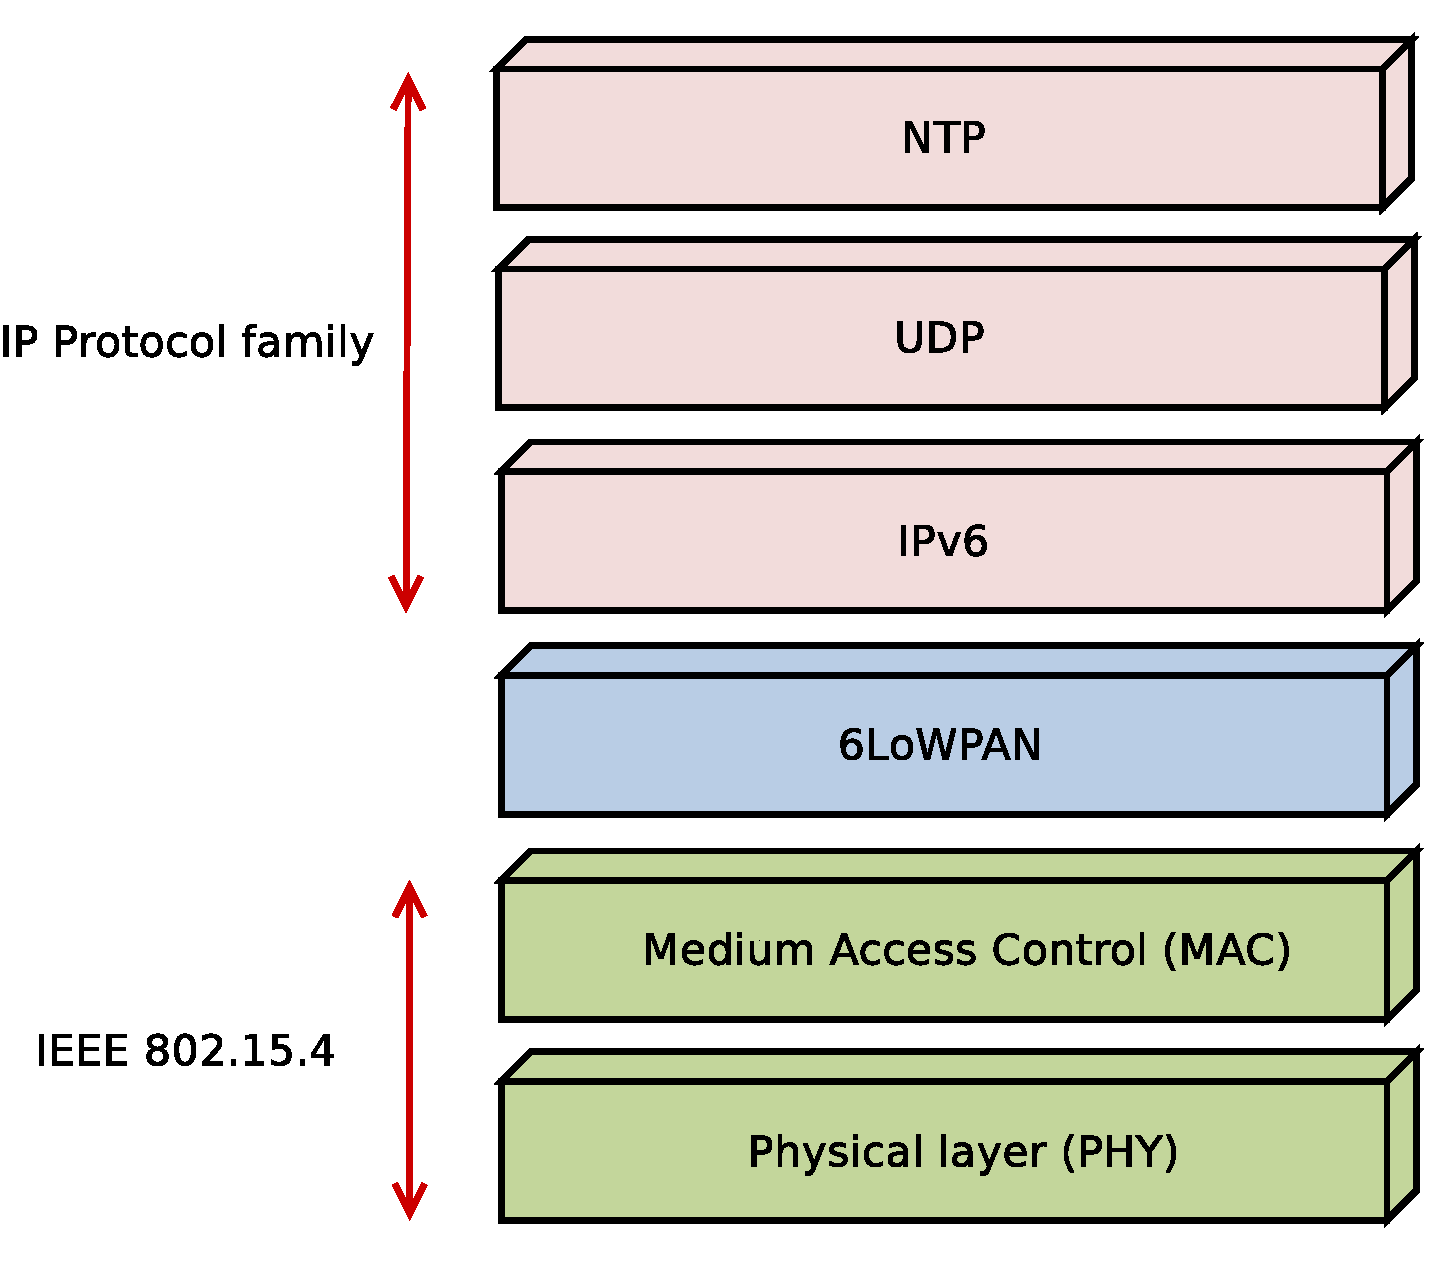
\includegraphics[width=9cm,keepaspectratio]{fig/6lowpan.pdf}
  \caption{Communication stack with 6lowpan layer}
  \label{fig:design-6lowpan}
  \bigskip
\end{figure}




%=========================================================================
% (c) 2011, 2012 Josef Lusticky

\section{Clock library extension}\label{sec:design-clock}
Previous section described how the call for getting the time acquires
the maximum precision the clock model allows.
Two read operations are needed in such a design - read {\it{scount}} and read {\it{TCNT2}}.
Since the {\it{scount}} variable depends on asynchronous interrupts produced by
the clock module, the followed query of the counter register causes a race condition.
The timer clock runs asynchronously from the CPU clock and
the result may be unpredictable if read while the timer is running.
Although the read could be wrapped with an interrupt disable,
the common solution on AVR platform in Contiki is to perform more read operations,
compare the results and perform read operations again if the results are not consistent.
Figure~\ref{fig:design-read} shows such a solution.

\begin{figure}
  \centering
  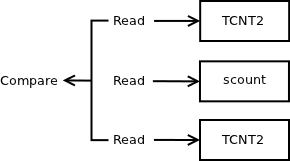
\includegraphics[width=6cm,keepaspectratio]{fig/read.png}
  \caption{Multiple read and result comparison}
  \label{fig:design-read}
\end{figure}

The call for adjusting the time computes the number of clock ticks
with the longer or shorter tick interval.
For storing the result, a new variable must be introduced.
If the value of this variable is zero, no adjustments are in progress.
Otherwise, the default value of the compare register is incremented or decremented by 1
and written to {\it{OCR2A}}.
This effectively causes adjusting the time, as described in section~\ref{sec:analysis-interface}.
When the time was adjusted enough,
the default value of the compare register is written back to {\it{OCR2A}}.

When adjusting the time in Contiki on AVR Raven, the as follows:
Section~\ref{sec:analysis-clock-interface} explained, that the default value
of the compare register for AVR Raven in Contiki is 31,
but the number of counter register increments between two successive interrupts is 32.
Incrementing the compare register value causes one real second to be experienced as
$\frac{f_{T2}}{CLOCK\_SECOND \times (32 + 1)} = \frac{4096}{128~\times~33} = 0.\overline{96}$~seconds
by the operating system.
Decrementing the compare register value causes one real second to be experienced as
$\frac{f_{T2}}{CLOCK\_SECOND \times (32 - 1)} = \frac{4096}{128~\times~31} \doteq 1.032258$~seconds
by the operating system.

Each increment of the counter register {\it{TCNT2}} takes
$\frac{1}{128 \times 32} = 0.000244140625$~seconds.
This is also the minimal possible clock adjustment,
that can be achieved by changing the compare register value just for one clock tick.
The fastest possible adjustment is approximately 0.03~$\frac{s}{s}$.
If faster adjustments were needed, the compare register would have to be updated with different values. 
However, updating the compare register with more different values would require
a more complicated software design
and lower values could cause a miss of the compare match described in section~\ref{sec:analysis-hwclock}.

% TO NTP INTERFACE
%When writing to compare register, the value is transferred to a
%temporary register, and latched after two positive edges of a source clock~\cite{avr-datasheet}.
%The user should not write a new value before the contents
%of the temporary register have been transferred to its destination.
%To detect that a transfer to the destination register has taken place,
%the Asynchronous Status Register - ASSR has been implemented.
%Since writing to compare register occurs only once within interrupt CONTEXT, % context?
%this detection is not mandatory.


%=========================================================================
% (c) 2011, 2012 Josef Lusticky

\section{Time interface extension}\label{sec:analysis-interface}
Section~\ref{sec:analysis-time} described, that there is no proper
way of setting, getting and adjusting the time for an NTP client in Contiki OS.
A new interface for setting, getting and eventually adjusting the time
must be therefore developed.

Setting the time should not cause a misbehaviour of the Contiki timers
described in section~\ref{sec:analysis-time}.
A modification of the {\it{scount}} and the {\it{seconds}} variable must be therefore avoided.
This can be achieved using an additional variable, containing the system boot time,
and modifying only that variable by the call for setting the time.
This way, the {\it{seconds}} variable will be further representing the system uptime
and the current real time can be obtained by $boottime + seconds$.
Since the {\it{scount}} also can not be changed, setting the time is only possible
within a precision of one second.
%Finer time setting must be made using the time adjustments.

By contrast, a call for getting the current time must be able to provide a higher precision.
Therefore, a new time specification structure must be designed as well.
To conform to the POSIX standard~\cite{posix}, this structure should consist of two parts -
one representing seconds and the other representing nanoseconds.
The first part represents the number of elapsed seconds since the POSIX epoch.
The nanosecond precision was chosen as modern systems also aim towards this
precision~\cite{posix,ntp-precision} and
the microsecond precision would also require at least 32-bit data type -
one second has 1~000~000 microseconds, which is more than the maximum expressible value of
an unsigned 16-bit data type $2^{16}$-1 (65~535).

The call for getting the time fills the time specification structure.
The part representing seconds is simply filled with the value of $boottime + seconds$,
while the part representing nanoseconds should be filled with the maximum precision
the clock model allows.
As described in section~\ref{sec:analysis-time},
this can be achieved by reading the {\it{scount}} variable
and by querying the hardware counter that is used for
interrupt generation and includes the time passed since
the last update of the {\it{scount}} variable.
This way, the resolution of
$\frac{1}{CLOCK\_SECOND~\times~counts} = \frac{1}{128~\times~32} = 0.000244140625$~seconds
can be acquired,
where $counts$ is the number of counter register increments between two successive interrupts,
which is 32 by default on AVR Raven, as stated in section~\ref{sec:analysis-clock-interface}.
%If this part was filled by only using the {\it{scount}} variable,
%just the resolution of the timer interrupt frequency would be provided.

Since setting the current time is possible only within one second precision,
finer time setting must be made using the time adjustments.
Section~\ref{sec:analysis-time} explained, that adjusting the time
should use the hardware clock as much as possible.
Adjusting the time changes the value in {\it{OCR2A}} compare register
to delay or shorten the clock tick interval,
which in turn speeds up or slows down the system time.
If the amount of required adjustments is positive, then the system clock is speeded up
until the adjustment has been completed.
If the amount of required adjustments is negative, then the clock is slowed down in a similar fashion.
Since the application specifies the amount of adjustments by the timestamp,
a new call must be developed for the determination of how many
clock ticks will be delayed or shortened, respectively.

As a result of this design, a leap second occurrence will be handled like an unexpected change of time -
the operating system will continue with the wrong system time for some time,
but an NTP client will set or adjust the system time~\cite{ntp-faq}.
This will effectively cause the leap second correction to be applied too late,
what is a trade-off for smaller memory requirements.


%%=========================================================================
% (c) 2011, 2012 Josef Lusticky

\section{Contiki NTP client}\label{sec:design-client}
The client application itself is a Contiki process,
which will use the designed operating system interface from the previous sections
and the uIP communication stack.

The client is able to use both NTP communication modes,
the NTP broadcast mode and the NTP unicast mode.
If the client will use only the broadcast mode, the structures and code
related to the unicast mode should not be included in the resulting program.
NTP broadcast mode packets can be received and processed from any NTP server in the network.
To avoid a complicated design when the NTP unicast mode is used,
the client is able to communicate only with one specified NTP server.

The NTP client fills and checks only the seconds part of the NTP timestamp,
because the conversion to the NTP format would increase the interval
between the timestamp determination and the dispatch of the filled packet.
After the filled NTP packet is sent, the client schedules
sending the next NTP packet in $2^{\tau}$ seconds %!LYDIA
by using the event timer library.
In NTPv4, $\tau$ ranges from 4, resulting in NTP poll interval of 16 seconds,
to 17, resulting in NTP poll interval of 36 hours.
However, the event timer library imposes a limit on the scheduled time.
This limit is platform specific and depends on the {\it{CLOCK\_SECOND}} value,
e.g. the $\tau$ value can not be greater than 8 on AVR Raven assuming 128 interrupts per second.
Upon scheduling the event timer, the client process yields
and another process could be run.
The client process is later invoked either by the uIP stack event
announcing the server response
or by the event timer in case no server response arrived.

Due to a missing simple solution for IPv4 communication over IEEE~802.15.4 link layer,
only IPv6 communication will be tested on the AVR Raven platform.
DNS resolution is not supported for this reason
and the remote server must be specified by address.

The packet loss problem was described in section~\ref{sec:analysis-application}.
However, a packet loss is not an issue if the client process uses the event timer library.
In the broadcast mode, a lost server packet causes no setting or adjusting the system time.
The client simply waits without disruption for the next NTP broadcast message.
If the client needs to figure out its local clock offset at the moment,
it can query the server by using the NTP unicast mode.
In the unicast mode, the client process is invoked in response to the expired event timer
and queries the server again.

When the server response arrives,
the destination timestamp determination is one of the first tasks the client does.
After that, the client makes packet sanity tests, including
checking whether the response is from a synchronised server.
In the unicast mode, the Originate Timestamp is compared with the stored sent timestamp. %!LYDIA
The received packet is considered bogus in case of a mismatch and further processing is stopped. %!LYDIA
Otherwise, the NTP timestamps are converted to the local timestamp format and
the local clock offset is computed as described in section~\ref{sec:ntp-algorithms}.
After the local clock offset is computed,
the stored transmitted timestamp is immediately set to zero
to protect against a replay of the last transmitted packet.
In the broadcast mode, the received packet is always considered correct
and the local clock offset is computed as the difference between the local stored timestamp
and the received Transmit Timestamp.
The local clock offset determined from the broadcast mode
is influenced by the network propagation delay and therefore less accurate.
The NTP client could exchange several packets with the server to calibrate the propagation delay.
But since local variables can not be reused in the Contiki process when the process yields,
this would cause either an extra memory overhead or a complicated client design.

Dynamic increasing or decreasing the client's Poll interval in response to
Kiss-o'-Death packets, described in section~\ref{sec:ntp-network}, would also
require a complicated design.
The client instead assumes, that an exhausted NTP server rather drops the incoming
client's query than sending a response with the KoD code.

Section~\ref{sec:design-interface} described that the client uses the POSIX timescale,
whereas NTP uses the NTP timescale.
Since both timescales reckon the time in seconds, %!LYDIA
the number of seconds between the NTP epoch and the POSIX epoch
can be simply subtracted from the seconds part of the NTP timestamp.
But the conversion from the fraction part of the long 64-bit NTP timestamp to nanoseconds,
used in the local timestamp structure,
is one of the most problematic tasks for memory constrained systems.
An accurate conversion requires either floating point operations or operations including 64-bit numbers~\cite{c99}.
The conversion is given by
$nsec = fractionl \times 10^9 \div 2^{32}$, where $nsec$ is the nanoseconds part of the local timestamp
and $fractionl$ is the fraction part of the long 64-bit NTP timestamp.

Because there is no native hardware support for floating point nor 64-bit arithmetic operations,
the compiler supplies these operations in form of library, called {\it{libgcc}} in case of the GCC compiler,
which causes a significantly bigger resulting binary file
(kilobytes in case of floating point operations and hundreds of bytes in case of 64-bit operations).
The greatest common divisor of $10^9$ and $2^{32}$ is $2^9$,
so in fact, a relatively simple multiplication of $fractionl$ by $\frac{5^9}{2^{23}}$ must be computed.
This could be computed on 32 bits using sequential
divisions by the power of 2 and multiplications by the power of 5.
In the standard C programming language, the bitwise right shift operator divides the unsigned data type by the power of 2
and the bitwise left shift operator multiplies the unsigned data type by the power of 2~\cite{c99}.
Therefore, the multiplication by 5 can be done using two left shifts and
adding the original value ($5x = 4x + x$).
The only constraint is that the overall coefficient of these operations must not be greater than 1,
that is, the value must be in the range from $0$ to $2^{32}-1$ in every step.
Otherwise, the value could overflow and the result would be incorrect.
Division can not cause such a situation but multiplication could.
The original value could be divided by a greater divisor,
but this would lead to a greater inaccuracy due to the lost of the least significant bits.
Because of this, multiplication done as soon as possible provides more accurate results.
The ideal conversion sequence is therefore given by formula~\ref{equ:conversion}.
\begin{equation}
\label{equ:conversion}
%\frac{10^9}{2^{32}} = \frac{2^9 \times 5^9}{2^9 \times 2^{23}} =
%\frac{5^9}{2^{23}} =
nsec = fractionl \times \frac{5}{2^3} \times \frac{5}{2^3} \times \frac{5}{2^3} \times \frac{5^2}{2^3} \times \frac{5}{2^3}  \times \frac{5}{2^3} \times \frac{5^2}{2^3} \times \frac{1}{2^2}
\end{equation}
It must be noted, that the above presented conversion is not exactly accurate,
because the least significant bits are lost by right shifts. %!LYDIA by
The accuracy can be determined by looping through all the possible values of $fractionl$ %!LYDIA by
and comparing the results with the reference algorithm that uses the floating point operations.
Such a measurement reports the maximum error of 5 nanoseconds,
which is totally adequate for most platforms without the floating point unit or
for platforms where 64-bit multiplication is expensive.
The implementation of the above as well as the program used for the
error measurement can be found on the CD attached to this thesis.
The table of CD contents is listed in appendix~\ref{app:cd-contents}.

After the timestamps were converted, the local clock offset is computed
as given in section~\ref{sec:ntp-algorithms}.
Depending on the absolute value of the local clock offset,
the system time is either set or adjusted using the {\it{clock\_set\_time}}
or {\it{clock\_adjust\_time}} call, respectively.
The clock is set if the time difference is equal or greater than
the offset threshold value.
The NTP specification suggests 0.125~seconds as the default~\cite{rfc5905}.
Because the designed call for setting the time, described in section~\ref{sec:design-interface},
can set the time only within a resolution of one second,
the threshold value must be at least one second.



%=========================================================================
% (c) 2011, 2012 Josef Lusticky <xlusti00@stud.fit.vutbr.cz>

\chapter{NTP client in Contiki OS}
%\!Distinguish between TIME and CLOCK

For implementation of a reasonably useful NTP client
operating system must meet conditions listed in appendix~\ref{app:requirements}.
The main problem for NTP client implementation in Contiki is a total
lack of time support.
Not only no common interface availability but also
almost no platform-specific code has been implemented towards time support yet.
Contiki provides basic clock interface particularly for use of timers though.
This interface is is common to for all supported platforms, but the particular implementation
is platform specific.

Another deal is possible packet loss if communication uses UDP on transport layer.
The reason while this can often happen is explained in section~\ref{sec:contiki-uip}.

For developing and testing Contiki NTP client the AVR Raven platform with CPU ATmega1284P was used.
How to get a working setup with Contiki on this platform is described in
%%% CHECK THIS %%%
docs/setup.pdf file on the CD enclosed to this thesis.
%%% CHECK THIS %%%

\section{Clock interface}
Contiki feature a basic clock interface with a simple goal - measuring time.
This interface provides needed calls for timers and its defintion is to be found in /core/sys/clock.h file.
Specific implementations of this common interface are localed in /cpu direcory of Contiki source code.
Interface provides call for initialising CPU's clock system - clock\_init, that is automatically called during
boot sequence of Contiki.
The goal of the clock\_init call is to set up
appropriate timer/counter registers and interrupt service routines.
On AVR CPUs this call is implemented as C macro which evaluates to specific setup code for each CPU
when compiling.
The setup code is not common to all CPUs because of differencies among them - e.g. there are usually
only three Timer/Counter modules, but AVR ATmega1284P has four Timer/Counter modules.

%At least one of those is always 16 bit wide
%This extra module on AVR ATmega1284P is used for
% three vs. 3

%clock\_seconds
%CLOCK\_SECOND
This is however enough for implementing a reasonable time interface and later using it for NTP client.

% ntp interface extending the clock library, similiar to posix calls

%\!!AVR


\section{NTP client implementation}
The structures representing NTP message were borrowed from OpenNTPD NTP Unix daemon.
%They are not using the GCC extension for representing a bit field.

A client sends messages to each server with a poll interval of $2^{tau}$
seconds, as determined by the poll exponent tau.
In NTPv4, $\tau$ ranges from 4 (16 s) to 17 (36 h).


\section{Network communication over UDP transport layer}
The uIP packet buffer is accessed through
the uip\_buf array and is used to hold incoming and outgoing packets.
The device driver should place incoming data into this buffer.
When sending data, the device driver should read the link
level headers and the TCP/IP headers from this buffer.
The size of the link level headers is configured by the UIP\_LLH\_LEN
define and in case of ethernet it is 14.

The application data need not be placed in this buffer, so
the device driver must read it from the place pointed to by the
uip\_appdata pointer %as illustrated by the following example:


%=========================================================================
% (c) 2011, 2012 Josef Lusticky

\chapter{Measurements}\label{chap:measurements}
There are several factors that can be measured.
Clock interrupt frequency measurements show the influence of clock adjustments
on the number of clock ticks (interrupts) per second.
Clock offset measurements show the time difference between the reference clock and
the local clock.
Clock phase measurements show the phase difference between the reference clock and
the local clock, that is, when each second is accounted.
The Meinberg~M600 NTP stratum 1 server was used as the reference clock
for all of the presented measurements.
The NTP client was running on the AVR Raven platform in a room with 23~\textcelsius
.

\section{Clock interrupt frequency}
For measuring clock interrupt frequency the bit 7 of Port D
and ground pin was connected to UNI-T~2025CEL digital oscilloscope.
At the beginning of the interrupt service routine a~logic 1 is written,
what causes a high level of voltage.
At the end of the interrupt service routine a~logic 0 is written,
what causes a low level of voltage.

When there is no clock adjustment, the value in output compare register is 31 by default.
The clock interrupt frequency
is supposed to be equal to a~value of the {\it{CLOCK\_SECOND}} macro, which is 128 by default on AVR~Raven.
The~figure~\ref{fig:app-osc-no-adjust} shows the output from oscilloscope
for this case.
$$\frac{\frac{f_{asy}}{prescaler}}{inc} = \frac{\frac{32768}{8}}{32} = 128$$

Figure~\ref{fig:app-osc-speed-up} shows the~output from oscilloscope
when slowing down the clock.
The~clock interrupt frequency
is supposed to be equal to $124.\overline{12}$~Hz.
$$\frac{\frac{f_{asy}}{prescaler}}{inc + 1} = \frac{\frac{32768}{8}}{32+1} = 124.\overline{12}$$

Figure~\ref{fig:app-osc-slow-down} shows the output from oscilloscope
when speeding up the clock.
The~clock interrupt frequency
is supposed to be approximately equal to 132.129~Hz.
$$\frac{\frac{f_{asy}}{prescaler}}{inc - 1} = \frac{\frac{32768}{8}}{32-1} \doteq 132.129$$

The~measured values are not exactly equal to those expected.
This is mostly due to influence of the clock source
(32~768~Hz quartz crystal oscillator) by a room temperature,
but it could also be air pressure or magnetic fields, etc.

\section{Clock offset}
\begin{figure}[H]
  \centering
  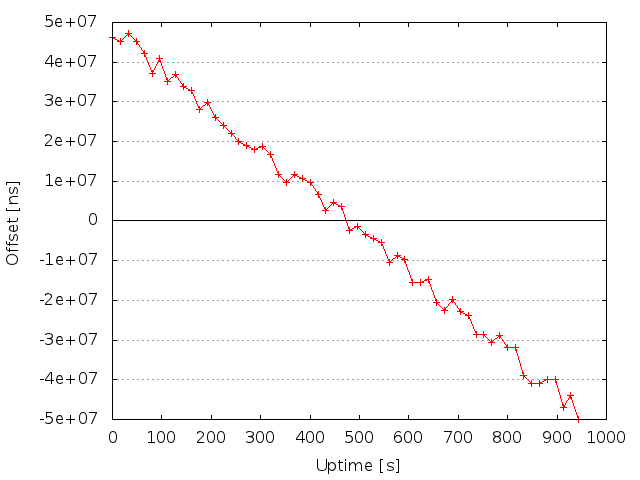
\includegraphics[width=11cm,keepaspectratio]{fig/no-ntp.png}
  \caption{Local clock offset without NTP client}
  \label{fig:measurements-no-ntp}
\end{figure}
Figure~\ref{fig:measurements-no-ntp} shows the local clock offset
in case no NTP client runs on the device.
The time is set with the initial offset of about 45 milliseconds.
However, the clock progresses faster due to frequency errors.
This compensate the initial clock offset at first,
but the local clock offset increases then.
Not only that the clock is running faster with approximately 100~PPM
(9 seconds a day) in this case,
but also the frequency jitter can be observed.
The offset increase is therefore not exactly linear.

Figure~\ref{fig:measurements-ntp-serial} shows the local clock offset
acquired from the serial output when Contiki NTP Client runs on the device.
When the developed NTP client receives response from the server,
it calculates the local clock offset and prints this value to the serial output.
The NTP poll interval was set to 16 seconds, that means, the local clock offset
is calculated and eventually corrected every 16 seconds.
\begin{figure}[H]
  \centering
  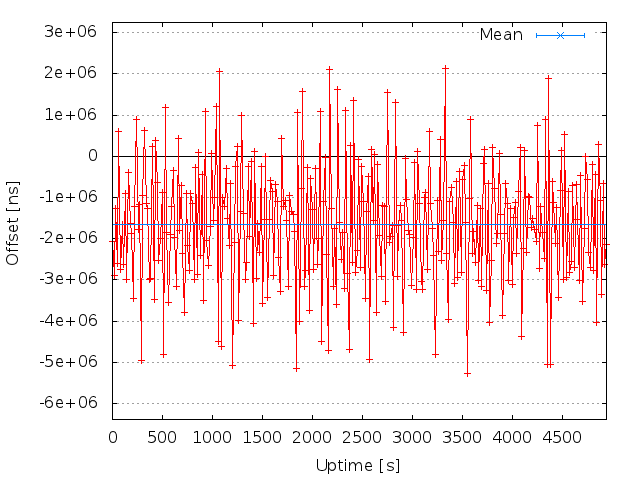
\includegraphics[width=11cm,keepaspectratio]{fig/poll-16s.png}
  \caption{Local clock offset with adjustments and NTP poll interval 16s}
  \label{fig:measurements-ntp-serial}
\end{figure}
The blue line shows the mean local clock offset value,
that should be equal to zero in a perfect case.
This is however not the case, because of oscillator frequency error
shown in figure~\ref{fig:measurements-no-ntp}.
More figures showing the local clock offset measurement
can be found in appendix~\ref{app:offset}.

\section{Clock phase}
The GPS based clock Meinberg~GPS~167 and digital oscilloscope UNI-T~2025CEL
was used for measuring the clock phase difference.
Meinberg~GPS clock rises an impulse when each second is accounted.
Contiki on AVR~Raven was configured to write a logic~1
to~bit~7 of~Port~D when each second is accounted,
and to write a logic~0 to~the same bit after~25 clock ticks.

When NTP client uses the {\it{clock\_adjust\_time}} call,
the local clock offset as well as the phase is being adjusted.
Figure~\ref{fig:measurements-osc-adjusting-phase} shows the phase while adjusting the clock.
The yellow line is the output signal from Meinberg~GPS clock
and the blue line is the output signal from AVR~Raven.
\begin{figure}[H]
  \centering
  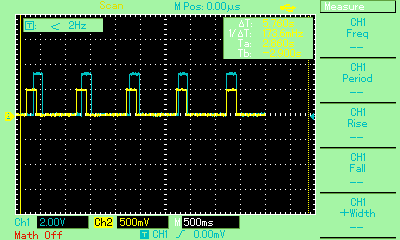
\includegraphics[width=11cm,keepaspectratio]{fig/osc-adjusting-phase.png}
  \caption{Second impulses when the clock is being adjusted}
  \label{fig:measurements-osc-adjusting-phase}
\end{figure}
Figures showing the clock out of phase and the clock in phase with
the reference clock can be found in appendix~\ref{app:phase}.


%! finish
\chapter{Conclusion}
The Network Time Protocol has been operating over 30 years as of early 2012
and remains the longest running, continuously operating application
protocol in the Internet~\cite{ntp-y2k}.
This thesis demonstrated, that its use can be further extended to a new platform of constrained devices,
such as embedded systems.

The developed NTP client for Contiki OS is able to use the NTP unicast and broadcast mode.
The implemented time interface extends Contiki OS towards real-time support,
while requiring minimal memory amounts.
The unique timestamp conversion provides a perfect solution to avoid the
memory expensive floating point or 64-bit arithmetic operations.
The measured results show that the Contiki NTP client is satisfying for keeping a reasonably accurate time.

The Network Time Protocol is suitable for constrained devices
forming the modern Internet and will arguably find its place among them in the near future.

%The implemented clock functionality




TODO - Future work:
It is useful to provide an initial volley where the client operating in
client mode exchanges several packets with the server, so as to
calibrate the propagation delay and to run the Autokey security
protocol, after which the client reverts to broadcast client mode~\cite{rfc5905}.

Refid~\cite{rfc5905}?? - not necessary

Ability to communicate with more servers. Requires clock selection algorithms.

Advanced clock discipline algorithms -
The clock discipline process is a system process that controls the
time and frequency of the system clock~\cite{rfc5905},

%Add timestamp into i-node in CFS.

%--
%ntpv4.pdf:
%SNTP is intended for primary
%servers equipped with a single reference clock, as well as clients with a single upstream server
%and no dependent clients.

%It is useful to provide an
%initial volley where the client operating in mode 3 exchanges several packets with the server in
%order to calibrate the propagation delay % ntp/algorithms.tex

%The operating system is assumed to provide two functions, one to set the time
%directly, for example the Unix settimeofday()1 function, and another to adjust the time in small
%increments advancing or retarding the time by a designated amount, for example the Unix
%adjtime() function. In the intended design the clock discipline process uses the adjtime() function
%if the adjustment is less than a designated threshold, and the settimeofday() function if above the
%threshold.

%An SNTP client using the on-wire protocol has a single server and no downstream clients. It can
%operate with any subset of the NTP on-wire protocol, the simplest using only the transmit
%timestamp of the server packet and ignoring all other fields. However, the additional complexity
%to implement the full on-wire protocol is minimal and is encouraged.


%--
%rfc5905:
%In the case of NTP as specified herein, NTP broadcast clients are
%vulnerable to disruption by misbehaving or hostile SNTP or NTP
%broadcast servers elsewhere in the Internet.  Such disruption can be
%minimized by several approaches.  Filtering can be employed to limit
%the access of NTP clients to known or trusted NTP broadcast servers.
%Such filtering will prevent malicious traffic from reaching the NTP
%clients.
 % viz. obsah.tex

  % Pouzita literatura
  % ----------------------------------------------
\ifczech
  \bibliographystyle{czechiso}
\else 
  \bibliographystyle{plain}
%  \bibliographystyle{alpha}
\fi
  \begin{flushleft}
  \bibliography{literatura} % viz. literatura.bib
  \end{flushleft}
  \appendix
  
  %=========================================================================
% (c) 2011, 2012 Josef Lusticky <xlusti00@stud.fit.vutbr.cz>

%\chapter{CD Content}
%\begin{tabular}{|l|l|}
	%\hline
	%Directory & Content \\ \hline
	%bib/ & Bibliography used in citations \\
	%\hline
%\end{tabular}

\chapter{Protothreads example}\label{app:protothreads}
Here is
%Next page shows
an example of delaying text on an LCD panel using Protothreads.
It is taken from
Adam Dunkel's Protothreads website~\cite{adam-protothreads} and slightly modified.
Protothreads can be used for introducing delays inside a function, without using a full threading model.
The example shows a function writing characters to LCD panel.
Suppose each character is shown for one second, then next character replaces previous.
\begin{lstlisting}
#include "pt.h"
#include "timer.h"

typedef unsigned short lc_t;

struct pt {
  lc_t lc;                                           /* Local continuation */
}; 

struct pt state;
struct timer timer;
 
PT_THREAD(display_text(struct pt *pt, const char *msg))
{
  PT_BEGIN(pt);
  for (int i = 0; i < strlen(msg); i++) {
    lcd_display_char(msg[i]);
    timer_set(&timer, ONE_SECOND);                 /* Wait for one second. */
    PT_WAIT_UNTIL(pt, timer_expired(&timer));
  }
  PT_END(pt);
}

int main(void)
{
  PT_INIT(&state);
  for (;;) {
    display_text(&state, "Hello world");
    /* Here can be another thread run */
  }
  return 0;
}
\end{lstlisting}
%\newpage
The PT\_WAIT\_UNTIL macro actually causes the function to return.
While the function is waiting for the timer to expire another function can be called and run.
When the function is entered again the execution continues with the PT\_WAIT\_UNTIL macro
which causes the function to check the condition it is waiting for (timer expired).
If the condition is met the function resumes, if not it returns again.
Strictly speaking the amount of time between showing each character can
be more than one second.
This is because Protothreads are not running simultenously: when the timer expires
and another Protothread is running, this Protothread would have to wait until
it is entered again. Than the condition specified in PT\_WAIT\_UNTIL is met and
next iteration of loop started, that is, next character is displayed.

How does it work? The macro PT\_BEGIN exapands to {\it switch} statement while preprocessing the
code for compilation.
The PT\_WAIT\_UNTIL macro expands to {\it case} and setting the local continuation
to the value, so that next time this function is run, it jumps to this {\it case}.
The structure holding the state is defined outside of the function so its context is not lost when
the function returns. The simplest state structure would hold just the local continuation variable.

Now follows the same sample of code after simplified preprocessing.
%Next page shows the same sample of code after simplified preprocessing.
%\newpage
\begin{lstlisting}
#include "pt.h"
#include "timer.h"

typedef unsigned short lc_t;

struct pt {
  lc_t lc;                                           /* Local continuation */
}; 

struct pt state;
struct timer timer;

int display_text(struct pt *pt, const char *msg)     /* Expanded PT_THREAD */
{
  switch(pt->lc) {  case 0:                      /* Expanded PT_BEGIN(pt); */
  
    for (int i = 0; i < strlen(msg); i++) {
      lcd_display_char(msg[i]);
      timer_set(&timer, ONE_SECOND);               /* Wait for one second. */
    
                                   /* The following two lines are expanded */
      pt->lc = 31; case 31:   /* PT_WAIT_UNTIL(pt, timer_expired(&timer)); */
      if(!(timer_expired(&timer))) { return PT_WAITING; }         /* macro */
    
    }
  
  pt->lc = 0; return PT_ENDED; }                        /* Expanded PT_END */
  
}

int main(void)
{
  state->lc = 0;                                       /* Expanded PT_INIT */
  for (;;) {
    display_text(&state, "Hello world");
    /* Here can be another thread run */
  }
  return 0;
}

\end{lstlisting}

\chapter{Requirements for NTP client and Contiki support}\label{app:requirements}
\begin{tabular}{|l|l|}
	\hline
	Requirement & Contiki support \\ \hline
	Communication using UDP & Complete \\
	DNS resolution & Missing IPv6, otherwise complete \\
	Setting the clock & Complete \\
	Adjusting the clock & None \\
	Setting the time & None \\
	Getting the time & None \\
	% Tomas Kasparek: semaphores, locks, ... ?
	\hline
\end{tabular}

\chapter{Overview of Abbreviations}
% Keep this sorted
\begin{tabular}{|l|l|l|}
	\hline
	Abbrevation & Meaning \\ \hline
	API & Application Programming Interface \\
	BSD & Berkeley Software Distribution \\
	CPU & Central Processor Unit \\
	DNS & Domain Name Resolution \\
%   EEPROM & Electrically Erasable Programmable Read-Only Memory \\
	GMT & Greenwich Mean Time \\
%	JTAG & Joint Test Action Group \\
	IETF & Internet Engineering Task Force \\
	ICMP & Internet Control Message Protocol \\
	IP & Internet Protocol \\
	LAN & Local Area Network \\
	NTP & Network Time Protocol \\
	POSIX & Portable Operating System Interface \\
	RAM & Random Access Memory \\
	RFC & Request for Comments \\
	SICS & Swedish Institute of Computer Science \\
	TCP & Transmission Control Protocol \\
	UDP & User Datagram Protocol \\
	UTC & Coordinated Universal Time \\
	\hline
\end{tabular}
 % viz. prilohy.tex
\end{document}
